%% ===========================================================================
%%  IR3C -- manuscript for Medical Image Analysis (Elsevier CAS double column)
%%  Build:  ./compile.sh   (regenerates tables and figures, then typesets)
%%  Every number in tables and figures is computed by scripts/make_tables.py and
%%  scripts/make_figures.py from archived per-volume results. Numbers quoted in the
%%  prose are cross-checked against scripts/numbers_digest.txt.
%%
%%  PENDING EXPERIMENTS: shaded table rows read "tbd"; boxed notes describe the protocol.
%%  Set \showpendingfalse to hide the boxed notes once the experiments are done.
%% ===========================================================================
\documentclass[a4paper,fleqn]{cas-dc}

\usepackage[authoryear]{natbib}
\usepackage{amsmath,amssymb}
\usepackage{booktabs}
\usepackage{colortbl}
\usepackage{multirow}
\usepackage{xspace}
\usepackage{tcolorbox}
\tcbuselibrary{breakable}
\usepackage{placeins}
\usepackage{float}

%% ---------------------------------------------------------------- pending markup
\newif\ifshowpending
\showpendingtrue
\definecolor{pendbg}{RGB}{255,243,224}
\definecolor{pendfg}{RGB}{154,91,18}
\definecolor{pendframe}{RGB}{224,160,80}
\newcommand{\tbd}{\textcolor{pendfg}{\textit{tbd}}}
\newcommand{\pendrow}{\rowcolor{pendbg}}
\newcommand{\pendlabel}{\textcolor{pendfg}{\textbf{[Pending experiment]}}}
\newcommand{\authorfill}[1]{\textcolor{pendfg}{\textbf{[#1]}}}
\newenvironment{pendingnote}[1]{%
  \ifshowpending
  \begin{tcolorbox}[breakable,colback=pendbg,colframe=pendframe,boxrule=0.5pt,arc=1pt,
    left=3pt,right=3pt,top=2pt,bottom=2pt,fontupper=\footnotesize,
    title={\footnotesize\bfseries To do before submission: #1},
    coltitle=pendfg,colbacktitle=pendbg,toptitle=1pt,bottomtitle=0pt]
  \else\setbox0\vbox\bgroup\fi}
  {\ifshowpending\end{tcolorbox}\else\egroup\fi}

\newcommand{\irthreec}{IR3C\xspace}
\newcommand{\Ithree}{I$^3$Net\xspace}

\begin{document}
\let\WriteBookmarks\relax
\def\floatpagepagefraction{1}
\def\textpagefraction{.001}

\shorttitle{Acquisition-conditioned reconstruction of missing and rejected MRI slices}
\shortauthors{[Authors]}

\title[mode=title]{Beyond uniform slice interpolation: acquisition-conditioned residual
correction for missing and rejected MRI slices}

\author[1]{[First author]}[orcid=0000-0000-0000-0000]
\cormark[1]
\ead{[email]}
\credit{[CRediT roles]}
\affiliation[1]{organization={[Institution]},
  city={[City]}, country={[Country]}}

\author[1]{[Second author]}
\credit{[CRediT roles]}

\cortext[1]{Corresponding author}

%% ---------------------------------------------------------------- abstract
\begin{abstract}
Learned through-plane MRI reconstruction is usually developed and tested on volumes in which
every $R$th slice is kept. In practice, the slices available for reconstruction may be
irregularly spaced, and slices corrupted by motion may be discarded after quality control.
Methods built around a fixed uniform grid then need a workaround before they can be applied.
We formulate the task as reconstruction from an arbitrary set of kept slices and propose
IR3C, a model that predicts a bounded correction to through-plane linear interpolation. The
network receives the sparse volume, its linear interpolant and four profiles computed from
the slice mask alone: whether a slice was kept, its relative position inside the gap, the gap
length and the distance to the nearest kept slice. Kept slices are copied to the output
exactly, and a zero-initialised output layer makes the untrained model equal to linear
interpolation. A single standard 3D U-Net serves all reduction factors and mask patterns. We
evaluate on brain T2-FLAIR (BraTS-GLI), brain T1-weighted (IXI-tiny) and knee DESS (OAIZIB)
MRI under uniform sampling, six irregular sampling families, an unseen reduction factor and
post-acquisition slice rejection, with every learned baseline trained under a matched budget.
On uniform sampling, the strongest specialist baseline, SAINT, is better at $R=2$ on all three
datasets, whereas IR3C is better at $R=8$. On irregular sampling, IR3C exceeds the strongest
applicable method by 2.2--3.0\,dB on BraTS-GLI, 0.9--1.7\,dB on OAIZIB and 1.4--2.9\,dB on
IXI-tiny. When 20--30\% of acquired slices are rejected, IR3C exceeds the best competitor,
including SAINT with two prespecified workarounds, by 1.2--2.3\,dB on both brain datasets.
IR3C also gives the highest whole-tumour agreement with the complete-input output of a frozen segmentation network at every factor, and reconstructs a volume in 0.26\,s. These results show that conditioning on the acquisition geometry and
correcting a deterministic estimate, rather than a new backbone, decide robustness once the
slice pattern departs from a uniform grid.
\end{abstract}

\begin{graphicalabstract}
%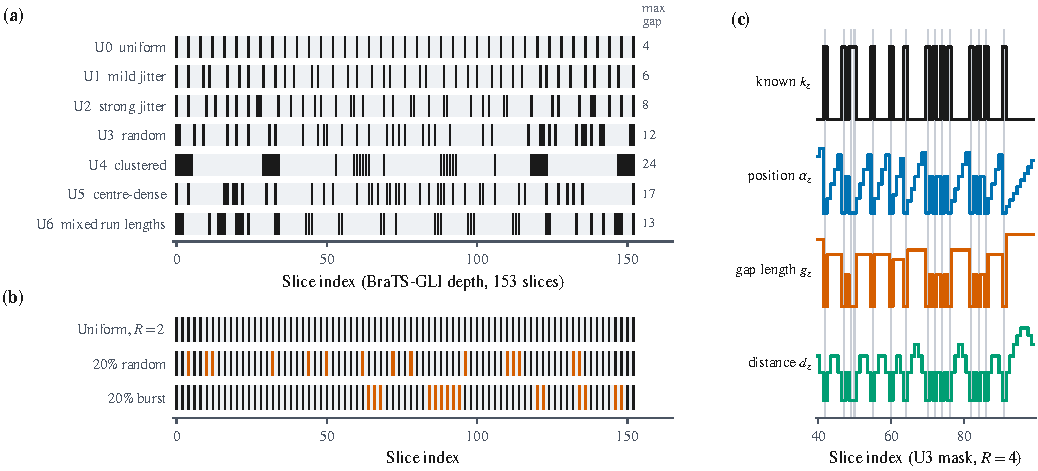
\includegraphics[width=\linewidth]{figs/fig1_sampling.pdf}
To be added
\end{graphicalabstract}

\begin{highlights}
\item Slice reconstruction is posed for arbitrary, irregular and rejected slice patterns
\item A linear anchor plus mask-conditioned bounded residual keeps acquired slices exact
\item Uniform-grid specialists win at low sparsity but lose once slices are rejected
\item One model serves all factors and patterns and is 5--55 times faster than baselines
\item Image-quality rankings and downstream segmentation consistency disagree
\end{highlights}

\begin{keywords}
MRI \sep missing-slice reconstruction \sep slice imputation \sep irregular sampling \sep
slice rejection \sep residual learning \sep robustness \sep downstream evaluation
\end{keywords}

\maketitle

%% ================================================================= 1 INTRODUCTION
\section{Introduction}
\label{sec:intro}

Many clinical MRI protocols acquire stacks of two-dimensional slices whose spacing is much
larger than the in-plane resolution. Downstream analysis, such as segmentation, registration
or volumetry, often requires values on a denser grid along the slice direction. Classical
interpolation fills the missing positions from neighbouring slices
\citep{lehmann1999interp}, and learned methods improve on it by exploiting anatomical
context \citep{chaudhari2018deepresolve,chen2018dcsrn,peng2020saint,song2024i3net}.

Most learned methods are developed on a regular grid. A dense reference volume is decimated
by keeping every $R$th slice, and the network is trained to restore the slices in between.
This benchmark is convenient and reproducible, but it fixes the geometry of the problem:
every gap has the same length, and the positions of the kept slices are known in advance.
Some architectures depend on this structure directly. SAINT, for example, splits a regular
stack into interleaved phases \citep{peng2020saint}, and \Ithree pads its input on the
assumption of a fixed stride \citep{song2024i3net}.

The slice pattern that a reconstruction method receives is not always uniform. Slice
positions vary between protocols and sites, archived volumes may contain gaps, and slices
degraded by motion or other artefacts may be rejected during quality control
\citep{zaitsev2015motion}. Outlier rejection is already an established step in
slice-to-volume reconstruction \citep{kuklisova2012outlier,kainz2015svr}. After rejection,
a method designed for a regular grid must either fill the rejected slices before inference
or discard further slices to recover a uniform subset. Both choices change the input that
the method was trained on.

The problem also provides a useful starting estimate. Linear interpolation along the slice
axis is exact at kept slices and gives a plausible low-frequency estimate between them. It
is defined for any slice pattern and costs almost nothing to compute. Residual learning for
MRI super-resolution is not new \citep{chaudhari2018deepresolve,peng2020saint}, and
arbitrary-scale methods based on implicit neural representations already accept
non-integer factors \citep{wu2023arssr,wang2024sainr}. Our question is narrower: can one
model, conditioned explicitly on the slice geometry and asked only to correct linear
interpolation, stay accurate when the slice pattern changes, including when acquired slices
are rejected?

We answer this question with IR3C, a deliberately simple method (Fig.~\ref{fig:arch}). The
network is a standard 3D U-Net \citep{ronneberger2015unet}. What changes is the task it is
given. The network receives the sparse volume, its linear interpolant and four
slice-geometry profiles derived from the mask alone. It predicts a bounded correction that
is applied only on missing slices, so kept slices are reproduced exactly. Because the output
layer is initialised to zero, the untrained model is exactly linear interpolation.

The contributions of this work are as follows.
\begin{enumerate}[(1)]
\item We formulate through-plane slice reconstruction for an arbitrary set of kept slices
and define the evaluated region, the slice geometry and the sampling conditions explicitly.
We separate uniform sampling, irregular sampling, unseen sparsity and post-acquisition slice
rejection as distinct test conditions.
\item We describe IR3C, a residual model anchored on linear interpolation and conditioned on
slice geometry. It keeps acquired slices exactly and uses one set of weights for all
reduction factors and sampling patterns.
\item We compare IR3C with four classical interpolants and four learned methods on three
datasets that differ in anatomy, contrast and slice geometry. All learned methods are trained
under a matched optimisation budget, and methods that are not defined on irregular grids are
evaluated through prespecified workarounds rather than omitted silently.
\item We report where IR3C does not win. A uniform-grid specialist is better at low
sparsity and on the dataset whose slice axis is already finely sampled. We also show that
image-similarity rankings and downstream segmentation consistency disagree.
\end{enumerate}

Throughout the paper, the degradation removes slices from a dense reference volume. This is
slice imputation, or missing-slice reconstruction. It does not model the slice profile,
partial-volume averaging or slice gap of a physically thick-slice acquisition
\citep{remedios2026eclare}, and we do not claim that the method restores thick-slice clinical
scans to isotropic resolution (Section~\ref{sec:limitations}).

%% ================================================================= 2 RELATED WORK
\section{Related work}
\label{sec:related}

\subsection{Learned through-plane reconstruction}

DeepResolve learned a residual mapping from thick-slice to thin-slice knee MRI and included a
reader study \citep{chaudhari2018deepresolve}. DCSRN used densely connected 3D convolutions
for brain MRI super-resolution \citep{chen2018dcsrn}. SAINT performs slice-wise
super-resolution on interleaved phases of a regular stack and then fuses the results with a
residual network \citep{peng2020saint}. \Ithree combines inter-slice and intra-slice branches
with cross-view processing \citep{song2024i3net}. SMORE trains on the target scan itself by
treating in-plane data as high-resolution examples \citep{zhao2021smore}. These methods
improve the quality of reconstruction on a regular grid. They do not address what happens
when the kept slices are irregularly spaced.

\subsection{Arbitrary-scale and acquisition-aware methods}

Implicit neural representations query intensities at continuous coordinates and therefore
accept arbitrary reduction factors. ArSSR learns such a representation for 3D MR images
\citep{wu2023arssr}, and SA-INR adds spatial attention for arbitrary reductions of slice
spacing \citep{wang2024sainr}. ECLARE models slice thickness, slice gap and field of view
explicitly for anisotropic resolution enhancement \citep{remedios2026eclare}. Our work is
complementary. We do not change the representation of the volume; we give an ordinary
convolutional network an explicit description of the local gap geometry, and we test what
this buys under irregular sampling and rejection.

\subsection{Imputation and physical thick-slice super-resolution}

Removing slices from an isotropic reference provides exact ground truth at every missing
position. It does not, however, simulate the through-plane point-spread function of a 2D
multi-slice acquisition. We therefore use the terms \emph{slice imputation} and
\emph{missing-slice reconstruction} for all experiments. Restoration of physically thick
slices would require slice-profile degradation or paired thin and thick acquisitions.

\subsection{Evaluation beyond image similarity}

PSNR and SSIM \citep{wang2004ssim} measure distortion but do not necessarily predict the
behaviour of a downstream analysis. Recent work reports imperfect agreement between
reconstruction metrics and downstream task performance \citep{wohlrapp2026downstream}.
Perceptual metrics such as LPIPS \citep{zhang2018lpips} rank methods differently again, in
line with the perception--distortion trade-off \citep{blau2018perception}. We therefore
report a downstream segmentation endpoint beside the image metrics and interpret LPIPS as a
secondary, descriptive measure.

%% ================================================================= 3 METHOD
\section{Problem formulation and method}
\label{sec:method}

\subsection{Problem formulation}
\label{sec:formulation}

Let $x\in[0,1]^{H\times W\times D}$ be a dense reference volume whose third axis is the
reconstruction axis, and let $\mathcal{K}\subset\{1,\dots,D\}$ be the set of kept slices,
with indicator $k_z=\mathbb{1}[z\in\mathcal{K}]$. The observation is
$x_s(:,:,z)=k_z\,x(:,:,z)$, and the missing-slice indicator is $m_z=1-k_z$. The task is to
estimate $x(:,:,z)$ for every $z$ with $m_z=1$, while reproducing kept slices unchanged. The
problem is posed in the image domain; raw k-space and coil data are not used.

A nominal reduction factor $R$ fixes the number of kept slices, $|\mathcal{K}|=\lceil (D-1)/R
\rceil+1$, so that all masks at the same $R$ contain the same amount of data and differ only
in where the slices are placed. The first and last slices are always kept, so no method has to
extrapolate. Training uses $R\in\{2,4,8\}$; $R=16$ is held out as an unseen level of sparsity.

\subsection{Sampling conditions}
\label{sec:families}

\paragraph{Sampling families.} We use seven mask families (Fig.~\ref{fig:sampling}a). U0 is
uniform decimation. U1 and U2 shift interior slices by small and large random offsets. U3
places interior slices at random. U4 clusters the kept slices into runs and leaves long gaps.
U5 samples the centre of the volume more densely than its ends. U6 mixes runs of different
lengths. All families keep the same number of slices at a given $R$. For testing, one mask is
generated per family and factor with a fixed seed and is shared by all subjects and methods.

\paragraph{Slice rejection.} To model rejection after quality control, a uniform acquisition
at base factor $R\in\{2,4\}$ loses a fraction $p\in\{0.1,0.2,0.3\}$ of its acquired interior
slices (Fig.~\ref{fig:sampling}b). In the \emph{random} pattern, slices are rejected
independently. In the \emph{burst} pattern, they are rejected in runs of two or three
consecutive acquired slices, as might follow a motion event. The rejection mask is generated
deterministically from the subject identifier, so each subject has its own mask, and the
same mask is given to every method.

\begin{figure*}[t]
\centering
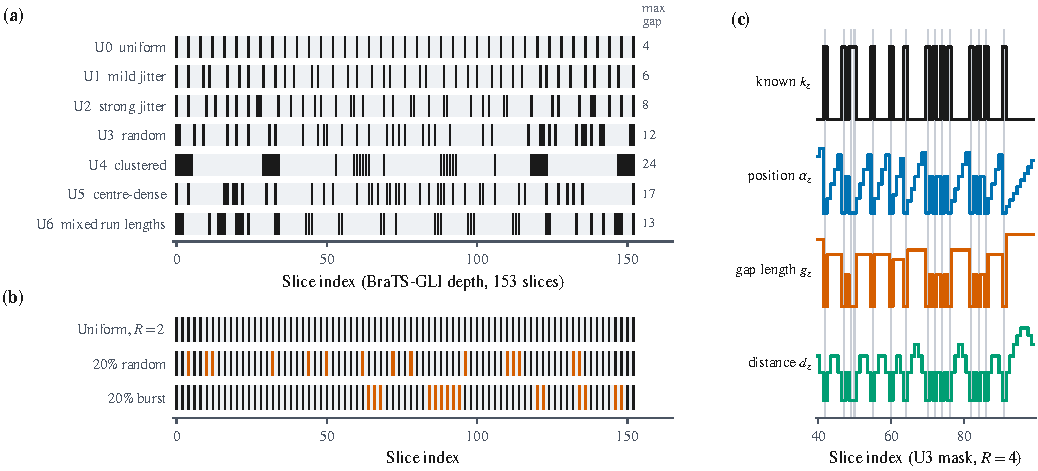
\includegraphics[width=\textwidth]{figs/fig1_sampling.pdf}
\caption{Sampling conditions studied in this work. (a)~The seven test-mask families at
$R=4$ on the 153-slice BraTS-GLI depth. Each tick is a kept slice; every family keeps 39
slices, so the families differ only in where the slices are placed. The number on the right
is the longest gap in slices. (b)~Slice rejection. A uniform $R=2$ acquisition loses 20\% of
its interior slices independently (random) or in runs of two to three slices (burst).
Black: acquired and kept; orange: acquired and rejected. (c)~The four geometry profiles that
IR3C receives, shown for a window of the U3 mask. Grey vertical lines mark kept slices.
Profiles are computed from the mask alone and are broadcast over the in-plane dimensions.}
\label{fig:sampling}
\end{figure*}

\subsection{IR3C}
\label{sec:ir3c}

\paragraph{Linear anchor.} For a missing slice $z$, let $l_z<z<r_z$ be the nearest kept
slices on either side. The anchor is through-plane linear interpolation,
\begin{equation}
\begin{gathered}
x_{\mathrm{lin}}(:,:,z)=(1-\alpha_z)\,x(:,:,l_z)+\alpha_z\,x(:,:,r_z),\\
\alpha_z=\frac{z-l_z}{r_z-l_z},
\end{gathered}
\label{eq:lin}
\end{equation}
and $x_{\mathrm{lin}}(:,:,z)=x(:,:,z)$ for kept slices.

\paragraph{Geometry profiles.} Four per-slice profiles describe the acquisition geometry
(Fig.~\ref{fig:sampling}c): the kept indicator $k_z$; the relative position $\alpha_z$; the
gap length $g_z=r_z-l_z$; and the distance to the nearest kept slice
$d_z=\min(z-l_z,\,r_z-z)$. Gap length and distance are log-compressed so that very long gaps
remain in a bounded range, $\tilde g_z=\log(1+g_z)/\log(161)$ and
$\tilde d_z=\log(1+d_z)/\log(81)$. All profiles except $k_z$ are zero on kept slices. Each
profile is broadcast over the in-plane dimensions. Together with $x_s$ and $x_{\mathrm{lin}}$,
the profiles form a six-channel input $X$. The profiles depend only on the mask, never on
image intensities.

\paragraph{Bounded residual.} A 3D U-Net $f_\theta$ maps $X$ to one channel. The
reconstruction is
\begin{equation}
\begin{gathered}
\hat x=\operatorname{clip}_{[0,1]}\!\bigl(x_{\mathrm{lin}}+m\odot s\tanh f_\theta(X)\bigr),\\
\hat x(:,:,z)\leftarrow x_s(:,:,z)\quad\text{if } k_z=1,
\end{gathered}
\label{eq:ir3c}
\end{equation}
where $m$ broadcasts the missing-slice indicator. The residual scale $s=0.585$ is fixed
before training as the 99.5th percentile of $|x-x_{\mathrm{lin}}|$ over foreground voxels of
missing slices in the training set. It limits how far the output can move from the anchor.
It does not guarantee that the corrected estimate is closer to the reference than linear
interpolation.

\paragraph{Initialisation and backbone.} The $1\times1\times1$ output layer is initialised to
zero, so the untrained model returns $x_{\mathrm{lin}}$ exactly. The backbone is a MONAI 3D
U-Net \citep{cardoso2022monai} with 32, 64, 128 and 256 channels, three stride-2
downsampling steps, two residual units per level, instance normalisation and PReLU
activations (4.75\,M parameters). We use a standard backbone on purpose: the backbone is the
implementation vehicle, not the contribution, and Section~\ref{sec:backbone} shows that the
results are not tied to it.

\begin{figure*}[t]
\centering
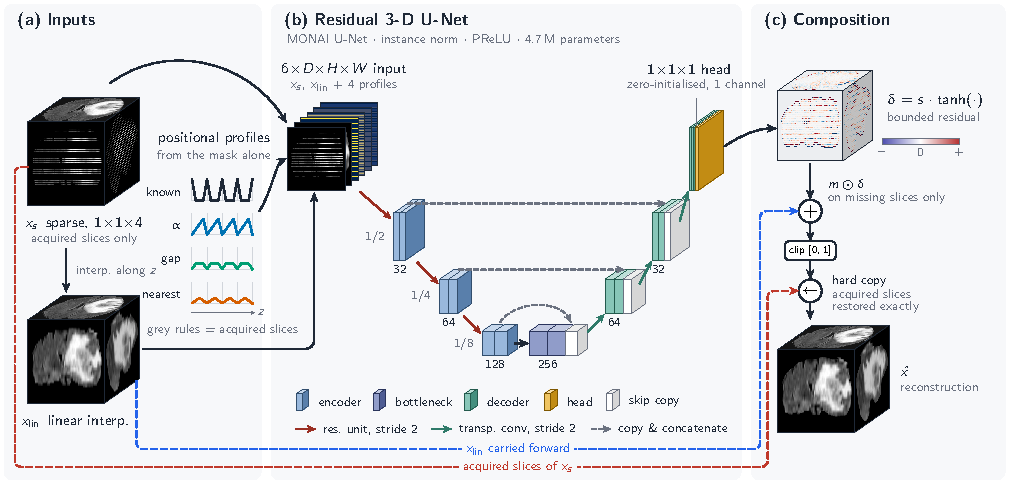
\includegraphics[width=\textwidth]{figs/fig_architecture3d.pdf}
\caption{IR3C. (a)~The sparse volume yields a linear through-plane anchor and four geometry
profiles computed from the slice mask alone. (b)~A standard 3D U-Net receives the six-channel
input and predicts one channel. (c)~The output is bounded by $s\tanh(\cdot)$, applied on
missing slices only and added to the anchor; acquired slices are copied to the output
exactly. Cube faces show an archived BraTS-GLI reconstruction.}
\label{fig:arch}
\end{figure*}

\subsection{Training objective}
\label{sec:loss}

The loss combines Charbonnier penalties \citep{charbonnier1997} inside and outside the
foreground mask, a structural term, a through-plane gradient term and a small penalty on the
residual:
\begin{equation}
\begin{aligned}
\mathcal{L}={}&\mathcal{L}_{\mathrm{C}}^{\mathrm{fg}}
+0.30\,\mathcal{L}_{\mathrm{C}}^{\mathrm{bg}}
+0.10\,\bigl(1-\mathrm{SSIM}\bigr)\\
&+0.05\,\mathcal{L}_{\nabla_z}^{\mathrm{fg}}
+0.001\,\lVert\delta\rVert_1,
\end{aligned}
\label{eq:loss}
\end{equation}
with $\delta=s\tanh f_\theta(X)$.
All terms are restricted to missing slices. The background term prevents the network from
adding low-level intensity outside the anatomy, which a foreground-only loss leaves
unconstrained. The contribution of each term is tested in Section~\ref{sec:pending-loss}.

%% ================================================================= 4 EXPERIMENTS
\section{Experimental setup}
\label{sec:setup}

\subsection{Datasets}
\label{sec:data}

Table~\ref{tab:datasets} summarises the three datasets. \emph{BraTS-GLI} (BraTS 2023 adult
glioma) provides co-registered, skull-stripped multi-contrast brain MRI
\citep{menze2015brats,bakas2017brats,baid2021brats}. We reconstruct the T2-FLAIR volume along
the axial axis. The 1251 subjects of the training release are used for training. Six
subjects of the validation release are used for checkpoint selection, and 88 further
validation-release subjects form the test set. BraTS-GLI is the development dataset and the
primary benchmark. \emph{OAIZIB} contains 507 knee DESS volumes from the Osteoarthritis
Initiative \citep{peterfy2008oai,ambellan2019oaizib}. We reconstruct along the sagittal
slice-select axis on the native grid and use the official 404/103 split, with 30 training
subjects held out for validation. \emph{IXI-tiny} contains 566 down-sampled T1-weighted brain
volumes derived from the IXI dataset \citep{ixi}. Its reconstruction axis is the axial axis,
which is also its finest axis (2.18\,mm). This makes IXI-tiny the dataset least suited to a
method that exploits a coarse slice direction.

Intensities are clipped to the 1st and 99.5th percentiles of the foreground and mapped to
$[0,1]$ once per volume; no slice-wise normalisation is applied.

\begin{table*}[t]
\caption{Datasets and subject-level partitions. ``Reconstruction axis'' is the axis along
which slices are removed; its number of slices $D$ and spacing are given. OAIZIB and
IXI-tiny models are fine-tuned on their own training partitions. Test subjects are never
used for training, early stopping or checkpoint selection.}
\label{tab:datasets}
\small
\begin{tabular*}{\textwidth}{@{\extracolsep{\fill}}lllllrrr@{}}
\toprule
Dataset & Anatomy, contrast & Grid (voxels) & Spacing (mm) & Reconstruction axis & Train & Val. & Test \\
\midrule
BraTS-GLI & Brain, T2-FLAIR & $240\times240\times153^{a}$ & $1.0\times1.0\times1.0$ & axial; $D=153$, 1.0\,mm & 1251 & 6 & 88 \\
OAIZIB & Knee, 3D DESS & $160\times384\times384$ & $0.70\times0.36\times0.36$ & sagittal; $D=160$, 0.70\,mm & 374 & 30 & 103 \\
IXI-tiny & Brain, T1-weighted & $83\times44\times55$ & $2.18\times4.13\times3.95$ & axial; $D=83$, 2.18\,mm$^{b}$ & 436 & 30 & 100 \\
\bottomrule
\end{tabular*}
\par\smallskip
{\footnotesize $^{a}$Central crop of the native 155 axial slices. $^{b}$The reconstruction
axis is the finest axis of this dataset, so $R=2$, 4 and 8 correspond to slice spacings of
4.36, 8.72 and 17.44\,mm.}
\end{table*}


\subsection{Comparators}
\label{sec:baselines}

\paragraph{Classical interpolation.} Nearest-neighbour, linear, global cubic-spline and local
bicubic interpolation along the reconstruction axis. The cubic spline is fitted along each
complete through-plane line and can overshoot when knots are irregular; bicubic uses a local
kernel.

\paragraph{Learned methods.} DCSRN \citep{chen2018dcsrn}, ArSSR \citep{wu2023arssr}, SAINT
\citep{peng2020saint} and \Ithree \citep{song2024i3net}. DCSRN is fully convolutional and is
trained on the same mixed uniform and irregular masks as IR3C, so it can be evaluated on
every family. ArSSR queries continuous coordinates and also accepts irregular masks. SAINT and
\Ithree construct their inputs from a regular stride. They are evaluated on U0, and under
rejection through the two workarounds described below; we do not assign them scores on
patterns for which their inference is undefined.

\paragraph{Matched budget.} All learned methods use the same subject partitions, masks,
intensity range and scored voxels. No baseline received more than 12,510 optimiser steps of
source training. IR3C is reported at the checkpoint reached after the same 12,510 steps
(``matched budget'') in every comparison, including the transfer datasets, where it is
fine-tuned from this checkpoint. The full 25-epoch IR3C model is reported only in
Appendix~\ref{app:budget}; it is 0.45\,dB better on BraTS-GLI, so the matched comparison is
conservative for IR3C. On OAIZIB and IXI-tiny, every learned method is fine-tuned on the same
target training split within the same target budget.

\paragraph{Workarounds under rejection.} SAINT and \Ithree receive two prespecified
workarounds when slices are rejected. In workaround A (\emph{imputation}), each rejected
slice is filled by linear interpolation from the surviving slices, and the model is run at
the original factor $R$. In workaround B (\emph{uniform subset}), the stride-$2R$ phase of the
original grid that lost fewer slices is selected, its rejected members are filled by linear
interpolation, and the model is run at factor $2R$. Every output, for every method, is
finally overwritten with the truly acquired slices, so all methods are scored on identical
missing slices.

\subsection{Evaluation protocol}
\label{sec:protocol}

PSNR is computed from the squared error pooled over all foreground voxels of the missing
slices of a volume. Kept slices are excluded, because every method copies them exactly and
including them would inflate all scores. SSIM \citep{wang2004ssim} is computed per missing
slice and averaged. NMSE and MAE use the same region. LPIPS \citep{zhang2018lpips} is
reported as a secondary metric in Appendix~\ref{app:detail}. This protocol was fixed before
the comparison and is applied identically to every method. It matters: in a separate check,
the same reconstruction scored between 26.0 and 46.0\,dB depending on the region,
normalisation and slice-wise versus volume-wise computation. Absolute values in this paper
should therefore not be compared with values reported elsewhere.

\subsection{Statistical analysis}
\label{sec:stats}

The subject is the unit of analysis. For each table row, a subject's cells (factors,
families or conditions) are averaged first, and the mean and standard deviation are then
computed across subjects. Paired comparisons use per-subject differences and report the mean
difference, its 95\% confidence interval from the $t$ distribution, the proportion of subjects
in which IR3C is better, and the two-sided Wilcoxon signed-rank test \citep{wilcoxon1945}.
Within each table, $p$-values are adjusted with the Holm procedure \citep{holm1979}. With 88
to 103 paired subjects, very small differences can be significant, so we interpret effect
sizes and confidence intervals rather than $p$-values alone.

\subsection{Downstream segmentation consistency}
\label{sec:downstream-setup}

A pretrained MONAI SegResNet \citep{myronenko2019segresnet,cardoso2022monai} for BraTS
receives the acquired T1, T1c and T2 volumes with either the complete or a reconstructed
FLAIR volume. The network is frozen and was never trained or tuned on any subject of this
study. Dice for whole tumour (WT), tumour core (TC) and enhancing tumour (ET) is computed
against the same network's prediction on the complete input. Because the test subjects come
from the BraTS validation release, which has no public labels, this endpoint measures how
much a reconstruction changes the output of a fixed pipeline. It does not measure
segmentation accuracy against expert labels.

\subsection{Implementation}
\label{sec:impl}

IR3C is trained on BraTS-GLI with AdamW (learning rate $2\times10^{-4}$, weight decay
$10^{-4}$), a 2\% linear warm-up followed by cosine decay, batch size 4, automatic mixed
precision and gradient clipping at 1.0. Training patches cover the full depth of the volume
so that every patch contains kept slices. For each training sample, $R$ is drawn from
$\{2,4,8\}$ with probabilities 0.30, 0.35 and 0.35; half of the samples use a uniform mask
and half use a fresh random mask from one of the six irregular families. Checkpoints are
selected on validation PSNR, subject to validation SSIM not falling more than 0.01 below that
of linear interpolation. For OAIZIB and IXI-tiny, the matched-budget BraTS-GLI model is
fine-tuned on the target training split, with the learning rate chosen by a short probe on
the target validation split and early stopping on validation PSNR. All experiments ran on a
single NVIDIA GB10 GPU.

%% ================================================================= 5 RESULTS
\section{Results}
\label{sec:results}

\subsection{Uniform sampling}
\label{sec:res-uniform}

Table~\ref{tab:uniform} and Fig.~\ref{fig:uniform} compare all methods on U0, where every
method is defined. The ranking depends on the reduction factor. At $R=2$, SAINT is the best
method on all three datasets; it exceeds IR3C by 0.81\,dB on BraTS-GLI, 0.37\,dB on OAIZIB and
3.70\,dB on IXI-tiny. At $R=8$, IR3C is the best method on all three datasets, by 0.98, 0.44 and
0.14\,dB, respectively, and it is better than SAINT in every BraTS-GLI and OAIZIB subject. At
$R=4$ the picture is mixed: IR3C is better on BraTS-GLI (0.46\,dB), the two methods are
practically equal on OAIZIB (0.01\,dB), and SAINT is better on IXI-tiny (2.02\,dB).

IXI-tiny is the clearest case in which IR3C does not win. Its reconstruction axis is already
the finest axis of the volume, so missing slices at $R=2$ and $R=4$ are spaced 4.4 and 8.7\,mm
apart and closely resemble their neighbours. This is the regime for which slice-wise
super-resolution on interleaved phases was designed. The other learned methods vary widely:
\Ithree is close to linear interpolation on both brain datasets, and ArSSR and DCSRN are
below linear interpolation at $R=2$ on BraTS-GLI. Among the methods that can be run on
irregular masks, IR3C is the best in every column of Table~\ref{tab:uniform}.

\begin{table*}[t]
\caption{Reconstruction on uniform sampling (U0). Values are means across test subjects; standard deviations are given in Appendix~\ref{app:detail}. Only missing slices inside the foreground mask are scored. Bold marks the best method per column. The paired row reports IR3C minus SAINT in dB; an asterisk marks $p<0.05$ (Wilcoxon signed-rank, Holm-corrected over the nine columns). Shaded rows are baselines that have not yet been run.}
\label{tab:uniform}
\small
\begin{tabular*}{\textwidth}{@{\extracolsep{\fill}}lccccccccc@{}}
\toprule
& \multicolumn{3}{c}{BraTS-GLI ($n=88$)} & \multicolumn{3}{c}{OAIZIB ($n=103$)} & \multicolumn{3}{c}{IXI-tiny ($n=100$)} \\
\cmidrule(lr){2-4}\cmidrule(lr){5-7}\cmidrule(lr){8-10}
Method & $R=2$ & $R=4$ & $R=8$ & $R=2$ & $R=4$ & $R=8$ & $R=2$ & $R=4$ & $R=8$ \\
\midrule
\multicolumn{10}{@{}l}{\textit{PSNR (dB) $\uparrow$}} \\
Linear & 30.17 & 26.33 & 22.11 & 21.03 & 19.00 & 17.53 & 28.17 & 22.52 & 18.53 \\
Bicubic & 30.46 & 26.53 & 22.12 & 20.77 & 18.70 & 17.22 & 29.07 & 22.68 & 18.37 \\
DCSRN & 19.73 & 22.53 & 20.27 & 20.58 & 19.40 & 18.13 & 23.53 & 20.85 & 16.85 \\
ArSSR & 25.07 & 23.79 & 21.43 & 21.75 & 20.46 & 19.12 & 26.32 & 23.80 & 21.41 \\
I$^3$Net & 30.37 & 26.32 & 22.12 & 22.02 & 20.26 & 18.98 & 28.63 & 22.72 & 18.95 \\
SAINT & \textbf{33.37} & 28.56 & 23.23 & \textbf{22.89} & 21.34 & 19.83 & \textbf{33.27} & \textbf{27.30} & 22.86 \\
\textbf{IR3C (ours)} & 32.56 & \textbf{29.01} & \textbf{24.21} & 22.52 & \textbf{21.35} & \textbf{20.27} & 29.57 & 25.27 & \textbf{23.00} \\
\pendrow SA-INR & \tbd & \tbd & \tbd & \tbd & \tbd & \tbd & \tbd & \tbd & \tbd \\
\pendrow 3D U-Net, direct output & \tbd & \tbd & \tbd & \tbd & \tbd & \tbd & \tbd & \tbd & \tbd \\
\midrule
\multicolumn{10}{@{}l}{\textit{SSIM $\uparrow$}} \\
Linear & 0.984 & 0.962 & 0.918 & 0.410 & 0.293 & 0.228 & 0.963 & 0.871 & 0.705 \\
Bicubic & 0.985 & 0.964 & 0.921 & 0.403 & 0.285 & 0.220 & 0.971 & 0.883 & 0.712 \\
DCSRN & 0.925 & 0.743 & 0.874 & 0.363 & 0.278 & 0.220 & 0.910 & 0.841 & 0.582 \\
ArSSR & 0.983 & 0.963 & 0.931 & 0.420 & 0.356 & 0.303 & 0.976 & 0.930 & 0.860 \\
I$^3$Net & 0.985 & 0.966 & 0.922 & 0.427 & 0.339 & 0.283 & 0.967 & 0.882 & 0.733 \\
SAINT & \textbf{0.991} & \textbf{0.975} & 0.935 & 0.473 & 0.393 & 0.328 & \textbf{0.990} & \textbf{0.956} & 0.876 \\
\textbf{IR3C (ours)} & 0.987 & 0.973 & \textbf{0.944} & \textbf{0.479} & \textbf{0.412} & \textbf{0.358} & 0.973 & 0.934 & \textbf{0.892} \\
\pendrow SA-INR & \tbd & \tbd & \tbd & \tbd & \tbd & \tbd & \tbd & \tbd & \tbd \\
\pendrow 3D U-Net, direct output & \tbd & \tbd & \tbd & \tbd & \tbd & \tbd & \tbd & \tbd & \tbd \\
\midrule
$\Delta$PSNR, IR3C $-$ SAINT & $-$0.81$^{\ast}$ & $+$0.46$^{\ast}$ & $+$0.98$^{\ast}$ & $-$0.37$^{\ast}$ & $+$0.01$^{\ast}$ & $+$0.44$^{\ast}$ & $-$3.70$^{\ast}$ & $-$2.02$^{\ast}$ & $+$0.14$^{\ast}$ \\
Subjects favouring IR3C (\%) & 27 & 74 & 100 & 0 & 59 & 100 & 0 & 0 & 63 \\
\bottomrule
\end{tabular*}
\end{table*}


\begin{figure*}[t]
\centering
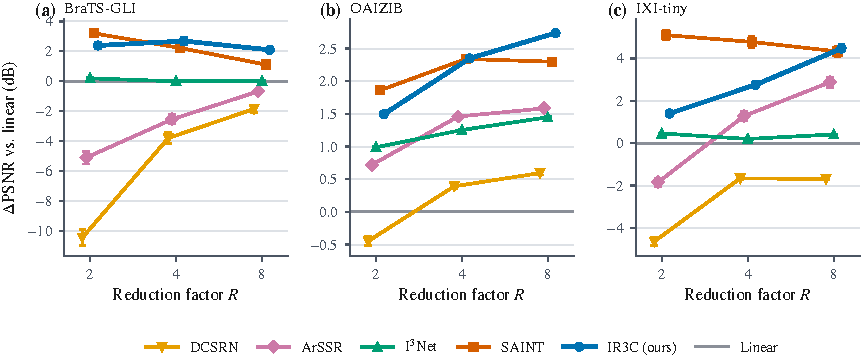
\includegraphics[width=\textwidth]{figs/fig3_uniform.pdf}
\caption{Uniform sampling (U0). PSNR difference from linear interpolation for each learned
method as a function of the reduction factor, on (a)~BraTS-GLI, (b)~OAIZIB and
(c)~IXI-tiny. Markers are means across test subjects; error bars are 95\% confidence
intervals of the paired difference. Markers are offset horizontally for legibility. Note the
different vertical scales.}
\label{fig:uniform}
\end{figure*}

\subsection{Irregular sampling}
\label{sec:res-families}

Table~\ref{tab:families} and Fig.~\ref{fig:families} report PSNR by sampling family. SAINT and
\Ithree are absent because they are not defined on irregular grids. On every family and
dataset, IR3C is better than every applicable method, and it is better in at least 99\% of
subjects in each column. On the irregular families U1--U6, its margin over the strongest
applicable comparator is 2.21--2.97\,dB on BraTS-GLI (over bicubic interpolation),
0.86--1.69\,dB on OAIZIB (over ArSSR) and 1.39--2.90\,dB on IXI-tiny (over ArSSR). The margin is
largest on the clustered family U4, which has the longest gaps, on all three datasets.

The classical methods behave differently from one another under irregular sampling. The
global cubic spline is close to linear interpolation on U0 but falls below it on every irregular family of every dataset, by up to 5.3\,dB on OAIZIB U4, because a spline through irregularly
spaced knots overshoots. Local bicubic interpolation remains close to linear interpolation.
Among the learned methods, DCSRN gains little over linear interpolation even though it was
trained on the same mixed masks as IR3C, which indicates that training on irregular masks
alone is not sufficient. The formulation ablation in Section~\ref{sec:pending-form} is
designed to separate the contributions of the anchor and of the geometry profiles.

\begin{table*}[t]
\caption{PSNR (dB) by sampling family, pooled over $R\in\{2,4,8\}$. U0 is uniform; U1--U6 are irregular (Section~\ref{sec:families}). I$^3$Net and SAINT are not defined off a regular grid and are therefore absent. The last row of each block is the paired difference between IR3C and the strongest applicable comparator in that column, with its 95\% confidence interval. Bold marks the best method per column. Standard deviations are given in Appendix~\ref{app:detail}.}
\label{tab:families}
\small
\begin{tabular*}{\textwidth}{@{\extracolsep{\fill}}lcccccccc@{}}
\toprule
Method & U0 & U1 & U2 & U3 & U4 & U5 & U6 & U1--U6 \\
\midrule
\multicolumn{9}{@{}l}{\textit{BraTS-GLI}} \\
Linear & 26.20 & 25.03 & 24.50 & 23.12 & 18.45 & 23.37 & 21.73 & 22.70 \\
Cubic spline & 26.32 & 24.96 & 24.36 & 22.53 & 17.01 & 22.96 & 20.82 & 22.10 \\
Bicubic & 26.37 & 25.17 & 24.61 & 23.17 & 18.46 & 23.42 & 21.78 & 22.77 \\
DCSRN & 20.84 & 20.64 & 20.34 & 19.78 & 17.02 & 19.77 & 18.83 & 19.40 \\
ArSSR & 23.43 & 22.95 & 22.65 & 21.94 & 18.14 & 21.98 & 20.51 & 21.36 \\
\textbf{IR3C (ours)} & \textbf{28.59} & \textbf{27.37} & \textbf{26.84} & \textbf{25.59} & \textbf{21.42} & \textbf{25.87} & \textbf{24.27} & \textbf{25.23} \\
\pendrow SA-INR & \tbd & \tbd & \tbd & \tbd & \tbd & \tbd & \tbd & \tbd \\
$\Delta$ vs.\ best comparator & $+$2.23 & $+$2.21 & $+$2.23 & $+$2.42 & $+$2.97 & $+$2.45 & $+$2.49 & $+$2.46 \\
\midrule
\multicolumn{9}{@{}l}{\textit{OAIZIB}} \\
Linear & 19.19 & 18.68 & 18.53 & 18.03 & 15.87 & 18.07 & 17.39 & 17.76 \\
Cubic spline & 18.63 & 17.71 & 17.24 & 15.45 & 10.57 & 14.67 & 14.29 & 14.99 \\
Bicubic & 18.90 & 18.41 & 18.27 & 17.79 & 15.71 & 17.83 & 17.18 & 17.53 \\
DCSRN & 19.37 & 18.98 & 18.84 & 18.35 & 16.38 & 18.40 & 17.81 & 18.13 \\
ArSSR & 20.44 & 20.13 & 19.99 & 19.39 & 16.90 & 19.49 & 18.78 & 19.11 \\
\textbf{IR3C (ours)} & \textbf{21.38} & \textbf{20.99} & \textbf{20.88} & \textbf{20.46} & \textbf{18.59} & \textbf{20.59} & \textbf{19.94} & \textbf{20.24} \\
\pendrow SA-INR & \tbd & \tbd & \tbd & \tbd & \tbd & \tbd & \tbd & \tbd \\
$\Delta$ vs.\ best comparator & $+$0.94 & $+$0.86 & $+$0.89 & $+$1.06 & $+$1.69 & $+$1.10 & $+$1.16 & $+$1.13 \\
\midrule
\multicolumn{9}{@{}l}{\textit{IXI-tiny}} \\
Linear & 23.07 & 21.45 & 21.56 & 19.93 & 14.56 & 19.25 & 18.73 & 19.25 \\
Cubic spline & 23.14 & 21.36 & 21.32 & 18.66 & 13.04 & 15.06 & 16.70 & 17.69 \\
Bicubic & 23.37 & 21.57 & 21.69 & 20.01 & 14.56 & 19.31 & 18.72 & 19.31 \\
DCSRN & 20.41 & 19.71 & 19.69 & 18.70 & 14.46 & 18.27 & 17.93 & 18.13 \\
ArSSR & 23.84 & 23.19 & 23.12 & 22.24 & 17.36 & 20.88 & 21.86 & 21.44 \\
\textbf{IR3C (ours)} & \textbf{25.95} & \textbf{24.66} & \textbf{24.69} & \textbf{23.90} & \textbf{20.26} & \textbf{22.89} & \textbf{23.25} & \textbf{23.27} \\
\pendrow SA-INR & \tbd & \tbd & \tbd & \tbd & \tbd & \tbd & \tbd & \tbd \\
$\Delta$ vs.\ best comparator & $+$2.11 & $+$1.47 & $+$1.57 & $+$1.66 & $+$2.90 & $+$2.01 & $+$1.39 & $+$1.83 \\
\bottomrule
\end{tabular*}
\end{table*}


\begin{figure*}[t]
\centering
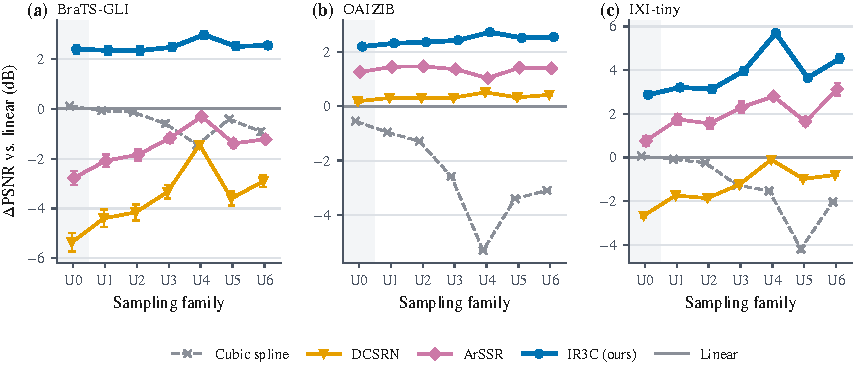
\includegraphics[width=\textwidth]{figs/fig4_families.pdf}
\caption{PSNR difference from linear interpolation by sampling family, pooled over
$R\in\{2,4,8\}$, on (a)~BraTS-GLI, (b)~OAIZIB and (c)~IXI-tiny. The shaded column is the
uniform family U0. Only methods that are defined on irregular grids are shown. Error bars are
95\% confidence intervals of the paired difference across subjects.}
\label{fig:families}
\end{figure*}

\subsection{Unseen sparsity}
\label{sec:res-r16}

No model was trained at $R=16$. Table~\ref{tab:r16} shows that IR3C remains the best method at
this factor on all datasets, pooled over all families (BraTS-GLI 18.22 versus 15.89\,dB for the
next best method; OAIZIB 16.99 versus 15.87\,dB; IXI-tiny 19.91 versus 16.99\,dB). Absolute
quality is low for every method, and in the most extreme cell (U4 at $R=16$ on BraTS-GLI,
where one gap spans most of the brain) no method recovers the anatomy. We therefore read this
result as graceful degradation outside the training range, not as a solution to extreme
sparsity.

\begin{table}[t]
\caption{Unseen sparsity, $R=16$ (never used in training). PSNR (dB), mean across test subjects. ``All'' pools U0--U6. DCSRN and I$^3$Net use factor-specific models and have no $R=16$ model; SAINT was not evaluated at this factor.}
\label{tab:r16}
\footnotesize\setlength{\tabcolsep}{3pt}
\begin{tabular*}{\columnwidth}{@{\extracolsep{\fill}}lcccccc@{}}
\toprule
& \multicolumn{2}{c}{BraTS} & \multicolumn{2}{c}{OAIZIB} & \multicolumn{2}{c}{IXI} \\
\cmidrule(lr){2-3}\cmidrule(lr){4-5}\cmidrule(lr){6-7}
Method & U0 & All & U0 & All & U0 & All \\
\midrule
Linear & 18.50 & 15.86 & 16.17 & 14.98 & 15.97 & 14.74 \\
Cubic spline & 18.24 & 14.43 & 15.54 & 11.60 & 15.32 & 12.67 \\
Bicubic & 18.33 & 15.74 & 15.86 & 14.74 & 15.72 & 14.55 \\
ArSSR & 18.70 & 15.89 & 17.47 & 15.87 & 18.44 & 16.99 \\
IR3C (ours) & \textbf{20.97} & \textbf{18.22} & \textbf{18.85} & \textbf{16.99} & \textbf{20.81} & \textbf{19.91} \\
\bottomrule
\end{tabular*}
\end{table}


\subsection{Slice rejection}
\label{sec:res-reject}

Table~\ref{tab:rejection} and Fig.~\ref{fig:rejection} report the rejection experiment.
Without rejection, the uniform-grid specialists retain their advantage where they had it on
U0: SAINT is better than IR3C at $R=2$ on BraTS-GLI and at both base factors on IXI-tiny.
Rejection reverses this ordering. On BraTS-GLI, IR3C is better than the strongest competitor
in every rejection condition, by 0.40--2.31\,dB. On IXI-tiny, the two methods are equal after
10\% random rejection at $R=2$ ($-0.02$\,dB, 95\% CI $-0.22$ to $0.18$), and IR3C is better in
every other rejection condition; after 20--30\% rejection its advantage is 1.22--2.16\,dB and
it is better in 92--100\% of subjects. The crossover therefore lies at about 10\% rejection
on both brain datasets.

The advantage grows with the rejected fraction and is larger for burst than for random
rejection, because bursts create longer gaps. The imputation workaround was the stronger of
the two SAINT workarounds in most conditions, but at 20--30\% rejection on IXI-tiny the
strongest competitor was ArSSR, which, like IR3C, accepts the irregular mask directly. Both
workarounds amount to presenting the specialist with an input that differs from its training
distribution: imputed slices are smooth linear estimates rather than acquired data, and the
uniform subset discards acquired slices. Fig.~\ref{fig:qual} shows the visible consequence on
a typical subject: horizontal discontinuities at the positions of rejected slices.

\begin{table*}[t]
\caption{Slice rejection. A uniform acquisition at base factor $R$ loses a fraction of its acquired interior slices, either independently (random) or in runs of two to three slices (burst). Each cell gives IR3C minus the strongest competitor in that condition (PSNR, dB) with its 95\% confidence interval; the strongest competitor is named underneath (A: rejected slices imputed linearly before inference; B: uniform stride-$2R$ subset). An asterisk marks $p<0.05$ after Holm correction over the conditions of one dataset. At 0\% the competitor runs in its native uniform regime. Absolute PSNR for every method is given in Appendix~\ref{app:reject}.}
\label{tab:rejection}
\small
\begin{tabular*}{\textwidth}{@{\extracolsep{\fill}}lllcccc@{}}
\toprule
Dataset & Base & Pattern & 0\% & 10\% & 20\% & 30\% \\
\midrule
BraTS-GLI & $R=2$ & random & $-$0.81 [$-$1.03, $-$0.60]$^{\ast}$ & $+$0.40 [0.22, 0.59]$^{\ast}$ & $+$1.20 [1.04, 1.36]$^{\ast}$ & $+$1.62 [1.49, 1.76]$^{\ast}$ \\
 & & & {\scriptsize\color{black!60}SAINT-A} & {\scriptsize\color{black!60}SAINT-A} & {\scriptsize\color{black!60}SAINT-A} & {\scriptsize\color{black!60}SAINT-A} \\[1pt]
 & $R=2$ & burst & $-$0.81 [$-$1.03, $-$0.60]$^{\ast}$ & $+$0.60 [0.45, 0.76]$^{\ast}$ & $+$1.29 [1.15, 1.43]$^{\ast}$ & $+$1.72 [1.59, 1.85]$^{\ast}$ \\
 & & & {\scriptsize\color{black!60}SAINT-A} & {\scriptsize\color{black!60}SAINT-A} & {\scriptsize\color{black!60}SAINT-A} & {\scriptsize\color{black!60}SAINT-A} \\[1pt]
 & $R=4$ & random & $+$0.46 [0.32, 0.59]$^{\ast}$ & $+$1.35 [1.23, 1.48]$^{\ast}$ & $+$1.76 [1.63, 1.89]$^{\ast}$ & $+$2.08 [1.95, 2.21]$^{\ast}$ \\
 & & & {\scriptsize\color{black!60}SAINT-A} & {\scriptsize\color{black!60}SAINT-A} & {\scriptsize\color{black!60}SAINT-A} & {\scriptsize\color{black!60}SAINT-A} \\[1pt]
 & $R=4$ & burst & $+$0.46 [0.32, 0.59]$^{\ast}$ & $+$1.55 [1.39, 1.71]$^{\ast}$ & $+$2.16 [1.97, 2.35]$^{\ast}$ & $+$2.31 [2.14, 2.48]$^{\ast}$ \\
 & & & {\scriptsize\color{black!60}SAINT-A} & {\scriptsize\color{black!60}SAINT-A} & {\scriptsize\color{black!60}SAINT-A} & {\scriptsize\color{black!60}SAINT-A} \\[1pt]
\midrule
OAIZIB & $R=2$ & random & $-$0.37 [$-$0.37, $-$0.36]$^{\ast}$ & $+$0.37 [0.35, 0.38]$^{\ast}$ & $+$0.78 [0.76, 0.80]$^{\ast}$ & $+$0.85 [0.82, 0.87]$^{\ast}$ \\
 & & & {\scriptsize\color{black!60}SAINT-A} & {\scriptsize\color{black!60}SAINT-A} & {\scriptsize\color{black!60}ArSSR} & {\scriptsize\color{black!60}ArSSR} \\[1pt]
 & $R=2$ & burst & $-$0.37 [$-$0.37, $-$0.36]$^{\ast}$ & $+$0.57 [0.54, 0.60]$^{\ast}$ & $+$0.89 [0.87, 0.91]$^{\ast}$ & $+$0.98 [0.95, 1.01]$^{\ast}$ \\
 & & & {\scriptsize\color{black!60}SAINT-A} & {\scriptsize\color{black!60}SAINT-A} & {\scriptsize\color{black!60}ArSSR} & {\scriptsize\color{black!60}ArSSR} \\[1pt]
 & $R=4$ & random & $+$0.01 [0.00, 0.02]$^{\ast}$ & $+$0.51 [0.48, 0.53]$^{\ast}$ & $+$0.93 [0.90, 0.96]$^{\ast}$ & $+$1.16 [1.12, 1.19]$^{\ast}$ \\
 & & & {\scriptsize\color{black!60}SAINT-A} & {\scriptsize\color{black!60}SAINT-A} & {\scriptsize\color{black!60}SAINT-A} & {\scriptsize\color{black!60}ArSSR} \\[1pt]
 & $R=4$ & burst & $+$0.01 [0.00, 0.02]$^{\ast}$ & $+$0.68 [0.64, 0.71]$^{\ast}$ & $+$1.17 [1.14, 1.20]$^{\ast}$ & $+$1.30 [1.26, 1.34]$^{\ast}$ \\
 & & & {\scriptsize\color{black!60}SAINT-A} & {\scriptsize\color{black!60}SAINT-A} & {\scriptsize\color{black!60}ArSSR} & {\scriptsize\color{black!60}ArSSR} \\[1pt]
\midrule
IXI-tiny & $R=2$ & random & $-$3.70 [$-$3.86, $-$3.53]$^{\ast}$ & $-$0.02 [$-$0.22, 0.18] & $+$1.22 [1.02, 1.42]$^{\ast}$ & $+$1.47 [1.34, 1.60]$^{\ast}$ \\
 & & & {\scriptsize\color{black!60}SAINT-A} & {\scriptsize\color{black!60}SAINT-A} & {\scriptsize\color{black!60}SAINT-B} & {\scriptsize\color{black!60}ArSSR} \\[1pt]
 & $R=2$ & burst & $-$3.70 [$-$3.86, $-$3.53]$^{\ast}$ & $+$0.78 [0.48, 1.09]$^{\ast}$ & $+$1.71 [1.55, 1.88]$^{\ast}$ & $+$1.70 [1.55, 1.84]$^{\ast}$ \\
 & & & {\scriptsize\color{black!60}SAINT-A} & {\scriptsize\color{black!60}SAINT-A} & {\scriptsize\color{black!60}ArSSR} & {\scriptsize\color{black!60}ArSSR} \\[1pt]
 & $R=4$ & random & $-$2.02 [$-$2.16, $-$1.88]$^{\ast}$ & $+$0.42 [0.25, 0.59]$^{\ast}$ & $+$1.64 [1.52, 1.76]$^{\ast}$ & $+$1.84 [1.70, 1.98]$^{\ast}$ \\
 & & & {\scriptsize\color{black!60}SAINT-A} & {\scriptsize\color{black!60}SAINT-A} & {\scriptsize\color{black!60}ArSSR} & {\scriptsize\color{black!60}ArSSR} \\[1pt]
 & $R=4$ & burst & $-$2.02 [$-$2.16, $-$1.88]$^{\ast}$ & $+$1.45 [1.19, 1.71]$^{\ast}$ & $+$1.92 [1.77, 2.07]$^{\ast}$ & $+$2.16 [1.98, 2.33]$^{\ast}$ \\
 & & & {\scriptsize\color{black!60}SAINT-A} & {\scriptsize\color{black!60}SAINT-A} & {\scriptsize\color{black!60}ArSSR} & {\scriptsize\color{black!60}ArSSR} \\[1pt]
\bottomrule
\end{tabular*}
\end{table*}


\begin{figure*}[t]
\centering
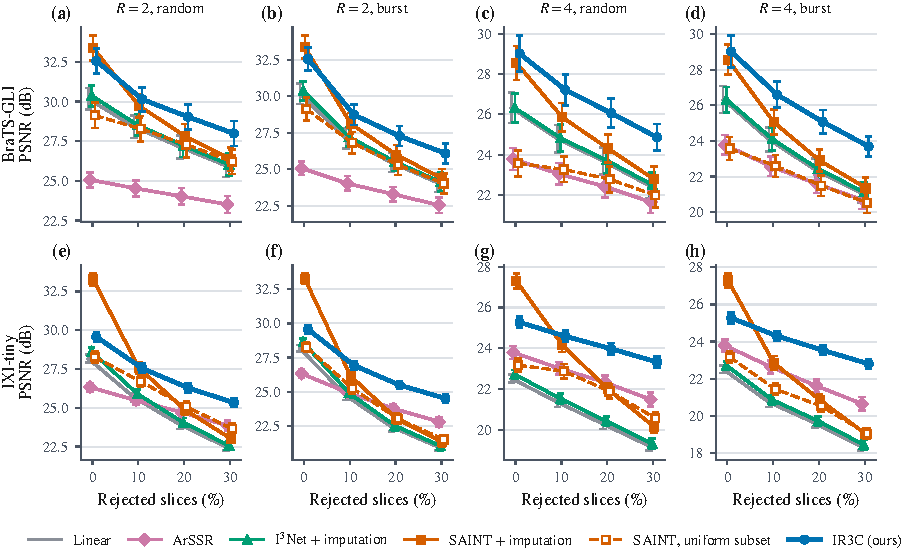
\includegraphics[width=\textwidth]{figs/fig5_rejection.pdf}
\caption{Slice rejection on BraTS-GLI (a--d) and IXI-tiny (e--h). PSNR on missing slices
against the fraction of acquired interior slices rejected, for base factors $R=2$ and $R=4$
and random or burst rejection. Error bars are 95\% confidence intervals of the cohort mean;
the paired differences, which are much tighter, are given in Table~\ref{tab:rejection}.
Markers are offset horizontally for legibility. DCSRN, bicubic interpolation and the \Ithree
uniform-subset workaround are omitted for clarity and are reported in
Appendix~\ref{app:reject}.}
\label{fig:rejection}
\end{figure*}

\begin{pendingnote}{OAIZIB slice rejection}
Run the OAIZIB arm of \texttt{IR3C\_SliceReject\_all} (it stopped after BraTS-GLI; smoke test
passed). It takes about 2.5 days on one GPU. It fills the shaded OAIZIB rows of
Table~\ref{tab:rejection} and adds a row to Fig.~\ref{fig:rejection}. This shows whether the
crossover also holds outside the brain.
\end{pendingnote}

\subsection{Downstream segmentation consistency}
\label{sec:res-downstream}

Table~\ref{tab:downstream} and Fig.~\ref{fig:downstream} report how far each reconstruction
moves the output of a frozen tumour segmentation network. The reference is the network's own
prediction on the complete input; re-saving and reloading the complete volume gives WT Dice
of 0.990, which is the noise floor of the pipeline. IR3C has the highest WT Dice at every factor and is best or within 0.001 of the best in every TC and ET column (WT 0.993, 0.985 and 0.961 at $R=2$, 4 and 8), and its advantage over linear
interpolation grows with sparsity (0.002, 0.007 and 0.013; Holm-adjusted $p<10^{-7}$ at every factor). The full-budget checkpoint changes WT Dice by at most 0.001, so this endpoint does not depend on the training budget. The classical interpolants stay close to IR3C on this endpoint even though they are
more than 2\,dB lower in PSNR.

The downstream ranking does not follow PSNR. SAINT is within 1\,dB of IR3C in PSNR on BraTS-GLI at
$R=4$ and $R=8$ (Table~\ref{tab:uniform}) but falls to WT Dice of 0.831 and 0.816. \Ithree,
whose PSNR is close to linear interpolation, falls further, to 0.676 and 0.646. The cause of
the SAINT drop is not yet established: its mean background intensity is low, so it does not
follow the background-haze mechanism we found for \Ithree, which shifts the intensity
normalisation of the segmentation network. Image metrics alone would not have revealed
these failures.

\begin{table*}[t]
\caption{Downstream segmentation consistency on BraTS-GLI (U0, $n=88$). A frozen SegResNet receives the acquired T1, T1c and T2 volumes with complete or reconstructed FLAIR. Dice is computed against the same network's prediction on the complete input, so it measures how far a reconstruction moves a fixed pipeline, not agreement with expert labels. Re-saving and reloading the complete volume gives WT/TC/ET Dice of 0.990/0.991/0.979, which is the pipeline's noise floor. WT: whole tumour; TC: tumour core; ET: enhancing tumour. $^{\dagger}$These reconstructions were archived from the full-budget IR3C checkpoint; the shaded row is the pending re-run with the budget-matched checkpoint used in all other tables.}
\label{tab:downstream}
\small
\begin{tabular*}{\textwidth}{@{\extracolsep{\fill}}lccccccccc@{}}
\toprule
& \multicolumn{3}{c}{WT Dice $\uparrow$} & \multicolumn{3}{c}{TC Dice $\uparrow$} & \multicolumn{3}{c}{ET Dice $\uparrow$} \\
\cmidrule(lr){2-4}\cmidrule(lr){5-7}\cmidrule(lr){8-10}
Method & $R=2$ & $R=4$ & $R=8$ & $R=2$ & $R=4$ & $R=8$ & $R=2$ & $R=4$ & $R=8$ \\
\midrule
Linear & 0.991 & 0.977 & 0.947 & 0.993 & 0.981 & 0.968 & 0.987 & 0.970 & 0.941 \\
Bicubic & 0.993 & 0.981 & 0.949 & \textbf{0.993} & 0.982 & 0.966 & 0.987 & 0.972 & 0.942 \\
DCSRN & 0.970 & 0.768 & 0.915 & 0.966 & 0.863 & 0.935 & 0.945 & 0.814 & 0.894 \\
ArSSR & 0.989 & 0.977 & 0.949 & 0.988 & 0.982 & \textbf{0.977} & 0.981 & 0.970 & 0.948 \\
I$^3$Net & 0.923 & 0.676 & 0.646 & 0.935 & 0.835 & 0.816 & 0.903 & 0.795 & 0.784 \\
SAINT & 0.986 & 0.831 & 0.815 & 0.980 & 0.894 & 0.871 & 0.961 & 0.852 & 0.828 \\
IR3C (ours)$^{\dagger}$ & \textbf{0.993} & \textbf{0.985} & \textbf{0.962} & 0.993 & \textbf{0.987} & 0.977 & \textbf{0.988} & \textbf{0.976} & \textbf{0.950} \\
\pendrow IR3C, matched budget & \tbd & \tbd & \tbd & \tbd & \tbd & \tbd & \tbd & \tbd & \tbd \\
\bottomrule
\end{tabular*}
\end{table*}


\begin{figure*}[t]
\centering
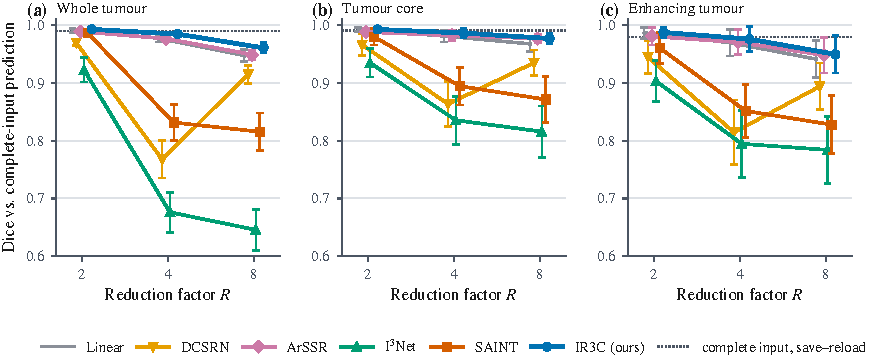
\includegraphics[width=\textwidth]{figs/fig6_downstream.pdf}
\caption{Downstream segmentation consistency on BraTS-GLI (U0, $n=88$). Dice between the
frozen network's prediction from reconstructed FLAIR and its prediction from complete FLAIR,
for (a)~whole tumour, (b)~tumour core and (c)~enhancing tumour. The dotted line is the Dice
obtained by re-saving and reloading the complete input. Error bars are 95\% confidence
intervals across subjects.}
\label{fig:downstream}
\end{figure*}


\subsection{Qualitative results}
\label{sec:res-qual}

Fig.~\ref{fig:qual} shows sagittal reformats along the reconstruction axis for one subject,
chosen by a fixed rule as the subject with the median IR3C gain among the five archived
showcase subjects. On uniform sampling, all learned methods reduce the stair-step appearance
of linear interpolation; SAINT and IR3C give the lowest error. After 30\% burst rejection,
the baselines show horizontal bands at the rejected positions, where gaps of up to 16 slices
are bridged by smooth interpolation. IR3C reconstructs these gaps with less banding and has
the lowest missing-slice error (MAE 0.065 versus 0.076 for SAINT with imputation).

\begin{figure*}[t]
\centering
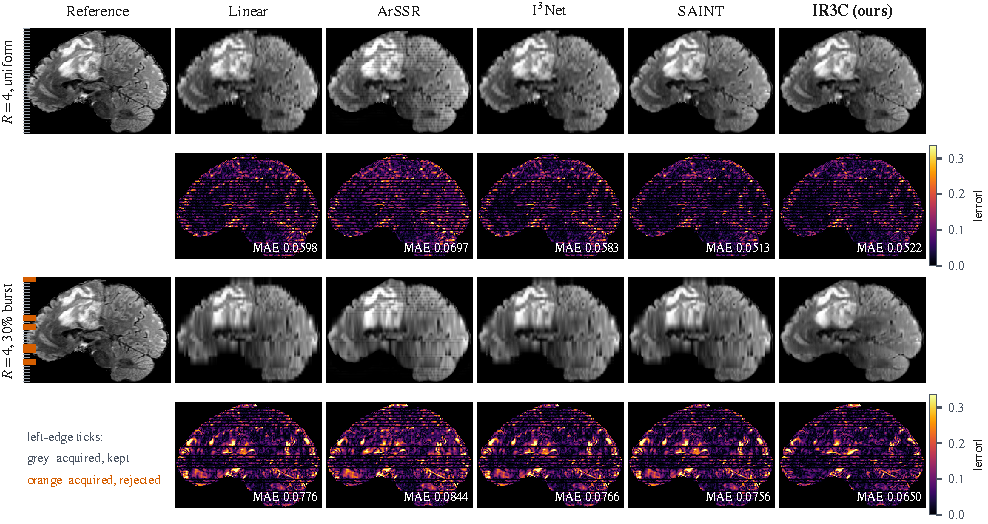
\includegraphics[width=\textwidth]{figs/fig7_qualitative.pdf}
\caption{Sagittal reformats of BraTS-GLI-00047-000 along the reconstruction axis (vertical).
Top two rows: uniform sampling at $R=4$. Bottom two rows: the same acquisition after 30\%
burst rejection. Error maps show absolute error on missing slices only (acquired slices are
exact for every method and are shown black); MAE is computed over the same voxels. Ticks on
the left edge of the reference mark kept (grey) and rejected (orange) acquired slices. All
images share one intensity window and all error maps share one scale. \Ithree and SAINT use
the imputation workaround in the rejection rows. The subject was selected by a rule fixed in
advance (median IR3C gain among five showcase subjects).}
\label{fig:qual}
\end{figure*}

\subsection{What makes the formulation work}
\label{sec:ablations}

\subsubsection{Choice of anchor}
\label{sec:anchor}

Table~\ref{tab:anchor} replaces the linear anchor with other interpolants while keeping the
initial weights and the order of training data fixed. The anchors differ by 2.60\,dB before
correction (20.69 to 23.28\,dB), but the corrected models differ by only 0.37\,dB (25.80 to
26.17\,dB). The best raw interpolant (bicubic) does not give the best final model; the linear
anchor does. The learned correction therefore absorbs most of the error of the starting
estimate, and a simple, exact-at-the-knots anchor is a sufficient starting point.

\begin{table}[t]
\caption{Choice of anchor (BraTS-GLI, all families, $R\in\{2,4,8\}$, $n=88$). Each model is trained from the same initial weights with identical data order; only the interpolant used as the anchor changes. $\Delta$ is the paired difference to the linear-anchored model with its 95\% confidence interval.}
\label{tab:anchor}
\footnotesize\setlength{\tabcolsep}{3pt}
\begin{tabular*}{\columnwidth}{@{\extracolsep{\fill}}lccc@{}}
\toprule
Anchor & Alone & Corrected & $\Delta$ vs.\ linear anchor \\
\midrule
Nearest & 20.69 & 25.80 & $-$0.37 [$-$0.40, $-$0.34] \\
Linear & 23.20 & 26.17 & --- \\
Cubic spline & 22.71 & 26.13 & $-$0.04 [$-$0.06, $-$0.01] \\
Bicubic & 23.28 & 26.05 & $-$0.12 [$-$0.14, $-$0.10] \\
\bottomrule
\end{tabular*}
\end{table}


\subsubsection{Backbone capacity}
\label{sec:backbone}

Table~\ref{tab:backbone} changes only the network that predicts the correction. A smaller
bottleneck costs 0.04\,dB. A depthwise-separable network with one fifth of the parameters
costs 1.17\,dB. An nnU-Net-configured backbone \citep{isensee2021nnunet} with 45\,M parameters
gains 1.51\,dB on irregular masks and is better for every subject, at about six times the
inference cost. The formulation is therefore not tied to one backbone, and its accuracy
improves with capacity. All rows use a single training seed.

\begin{table}[t]
\caption{Backbone capacity (BraTS-GLI, $R\in\{2,4,8\}$, $n=88$, single seed). The anchor, input profiles, loss and training budget are identical; only the network that predicts the correction changes. $\Delta$ is the paired difference to the IR3C backbone on U1--U6. Parameter counts and multiply--accumulate operations (MACs) are for one full-volume forward pass.}
\label{tab:backbone}
\footnotesize\setlength{\tabcolsep}{3pt}
\begin{tabular*}{\columnwidth}{@{\extracolsep{\fill}}lccccc@{}}
\toprule
Backbone & Param.\ (M) & GMACs & U0 & U1--U6 & $\Delta$ \\
\midrule
MONAI U-Net (IR3C) & 4.75 & 218 & 29.07 & 25.69 & --- \\
Reduced bottleneck & 3.63 & 198 & 29.00 & 25.65 & $-$0.04 \\
Depthwise separable & 0.98 & 41 & 27.59 & 24.51 & $-$1.17 \\
nnU-Net config. & 45.44 & 2434 & 31.25 & 27.20 & $+$1.51 \\
\bottomrule
\end{tabular*}
\end{table}


\subsubsection{Formulation ablation}
\label{sec:pending-form}

The experiments above show the performance pattern of IR3C but do not show which part of the
formulation produces its robustness. Table~\ref{tab:formulation} is designed to answer this
with the backbone, optimiser and budget held fixed. The key comparisons are the same network
predicting the image directly (no anchor), the anchored model without geometry profiles, and
the anchored model trained on uniform masks only. If robustness comes from anchoring and
geometry conditioning rather than from the backbone, the direct model and the model without
profiles should lose most of IR3C's advantage on U1--U6, on U4 and under rejection, while
remaining competitive on U0.

\begin{table*}[t]
\caption{\pendlabel\ Formulation ablation on BraTS-GLI with the backbone, optimiser and training budget held fixed. PSNR (dB) on test subjects, $R\in\{2,4,8\}$ unless stated; the rejection column is $R=4$ with 30\% burst rejection. Arms named in typewriter font are already packaged for the HPC run (Section~\ref{sec:pending-form}); ``new arm'' must be added. Values for multi-seed arms are to be reported as mean $\pm$ standard deviation over seeds. Only the linear row is computed.}
\label{tab:formulation}
\footnotesize\setlength{\tabcolsep}{3pt}
\begin{tabular*}{\textwidth}{@{\extracolsep{\fill}}llccccccc@{}}
\toprule
Variant & Arm & Seeds & U0 & U1--U6 & U4 & $R=16$ & Rejection & $\Delta$ vs.\ IR3C (U1--U6) \\
\midrule
Linear interpolation only & --- & --- & 26.20 & 22.70 & 18.45 & 15.86 & \tbd & --- \\
\pendrow Direct 3D U-Net (no anchor) & \texttt{A3\_direct} & 3 & \tbd & \tbd & \tbd & \tbd & \tbd & \tbd \\
\pendrow Anchor, unbounded residual & \texttt{A1\_unbounded} & 1 & \tbd & \tbd & \tbd & \tbd & \tbd & \tbd \\
\pendrow Anchor, non-zero output head & \texttt{A2\_nonzero\_init} & 1 & \tbd & \tbd & \tbd & \tbd & \tbd & \tbd \\
\pendrow Anchor, no geometry profiles & \texttt{C2\_no\_positional} & 3 & \tbd & \tbd & \tbd & \tbd & \tbd & \tbd \\
\pendrow Anchor, binary mask profile only & new arm & 1 & \tbd & \tbd & \tbd & \tbd & \tbd & \tbd \\
\pendrow Anchor, uniform-only training & \texttt{C1\_uniform\_only} & 1 & \tbd & \tbd & \tbd & \tbd & \tbd & \tbd \\
\pendrow Anchor, single factor ($R=4$) & \texttt{C3\_single\_R} & 1 & \tbd & \tbd & \tbd & \tbd & \tbd & \tbd \\
\pendrow IR3C (full formulation) & \texttt{A0\_ir3c} & 3 & \tbd & \tbd & \tbd & \tbd & \tbd & --- \\
\bottomrule
\end{tabular*}
\end{table*}


\begin{pendingnote}{formulation ablation (Table~\ref{tab:formulation})}
Seven of the eight arms already exist in the HPC package
\texttt{hpc\_ir3c\_ablations\_v2.tar.gz} (\texttt{A0}--\texttt{A3}, \texttt{C1}--\texttt{C3};
see \texttt{HANDOVER\_IR3C\_ABLATIONS.md}). Two additions are needed: (i)~a new arm that keeps
only the binary kept-slice profile $k_z$, and (ii)~seeds 43 and 44 for \texttt{A0\_ir3c},
\texttt{A3\_direct} and \texttt{C2\_no\_positional}. Evaluate every arm on the BraTS-GLI test
masks, at $R=16$, and on the rejection condition $R=4$, 30\% burst. The loss-term arms
\texttt{B1}--\texttt{B3} are reported separately in Table~\ref{tab:loss}. Report
\texttt{A1\_unbounded} as it is, even if it diverges.
\end{pendingnote}

\subsubsection{Loss terms}
\label{sec:pending-loss}

Table~\ref{tab:loss} removes one term of Eq.~(\ref{eq:loss}) at a time, with the backbone,
initial weights, data order and budget held fixed, and scores each model on image metrics
and on downstream segmentation consistency. The background term is the main test case. It
acts only outside the anatomy, where PSNR is not measured, so removing it should cost little
PSNR. If the network then adds low-level intensity to the background, the intensity
normalisation of the segmentation network shifts, and Dice should fall, as it does for
\Ithree\ (Section~\ref{sec:res-downstream}). The structural and gradient terms are expected
to have smaller effects on both endpoints.

\begin{table*}[t]
\caption{\pendlabel\ Loss-term ablation on BraTS-GLI: each arm removes one term of Eq.~(\ref{eq:loss}) and keeps everything else, including the $0.001\,\lVert\delta\rVert_1$ term, the backbone, the initial weights, the data order and the budget. PSNR (dB) is over missing-slice foreground, $R\in\{2,4,8\}$. Background haze is the mean predicted intensity on missing-slice background voxels, U0 ($\times10^{-3}$). WT Dice is the downstream consistency of Table~\ref{tab:downstream} (U0, $n=88$). The control \texttt{B0\_ir3c} is the same trained model as \texttt{A0\_ir3c} in Table~\ref{tab:formulation}. Only the linear row is computed.}
\label{tab:loss}
\small
\begin{tabular*}{\textwidth}{@{\extracolsep{\fill}}lllccccccc@{}}
\toprule
& & & \multicolumn{2}{c}{PSNR $\uparrow$} & Bg.\ haze $\downarrow$ & \multicolumn{3}{c}{WT Dice $\uparrow$} \\
\cmidrule(lr){4-5}\cmidrule(lr){7-9}
Variant & Arm & Removed term & U0 & U1--U6 & U0 & $R=2$ & $R=4$ & $R=8$ \\
\midrule
Linear interpolation only & --- & --- & 26.20 & 22.70 & 1.38 & 0.991 & 0.977 & 0.947 \\
\pendrow Full objective (Eq.~\ref{eq:loss}) & \texttt{B0\_ir3c} & --- & \tbd & \tbd & \tbd & \tbd & \tbd & \tbd \\
\pendrow No background term & \texttt{B1\_no\_background} & $0.30\,\mathcal{L}_{\mathrm{C}}^{\mathrm{bg}}$ & \tbd & \tbd & \tbd & \tbd & \tbd & \tbd \\
\pendrow No structural term & \texttt{B2\_no\_structure} & $0.10\,(1-\mathrm{SSIM})$ & \tbd & \tbd & \tbd & \tbd & \tbd & \tbd \\
\pendrow No gradient term & \texttt{B3\_no\_gradient} & $0.05\,\mathcal{L}_{\nabla_z}^{\mathrm{fg}}$ & \tbd & \tbd & \tbd & \tbd & \tbd & \tbd \\
\bottomrule
\end{tabular*}
\end{table*}


\begin{pendingnote}{loss-term ablation (Table~\ref{tab:loss})}
The three arms \texttt{B1\_no\_background}, \texttt{B2\_no\_structure} and
\texttt{B3\_no\_gradient} are already defined in the HPC package
(\texttt{ir3c\_ablations\_v2/arms.py}, Ablation~B) and will be trained locally with the
formulation ablation. The residual term ($0.001\,\lVert\delta\rVert_1$) is kept in every
arm. The control \texttt{B0\_ir3c} is \texttt{A0\_ir3c}, not a new training. Evaluate every
arm on the BraTS-GLI test masks and run the downstream segmentation of
Table~\ref{tab:downstream} (U0, $R\in\{2,4,8\}$, $n=88$) on each.
\end{pendingnote}

\subsection{Generalisation to unseen sampling geometry}
\label{sec:pending-heldout}

The irregular families used at test time are also used, with different random seeds, during
training. Results on U1--U6 therefore show robustness across the trained distribution of
masks, not generalisation to an unseen geometry. Only $R=16$ and the subject-specific
rejection masks lie outside the training distribution. We address this in three ways. Two
are still planned: leave-one-family-out training (Table~\ref{tab:heldout}) and several mask
realisations per subject instead of one shared mask (Table~\ref{tab:realisations}). The third
is done: an analysis of error against the local geometry of each missing slice
(Fig.~\ref{fig:gap}). It turns the named families into a statement about gap length and
distance to the nearest kept slice, which applies to any mask.

For every missing slice of the 88 BraTS-GLI test subjects we stored the foreground squared
error and voxel count under the 21 U0--U6 test masks ($R\in\{2,4,8\}$) and the 12 BraTS
rejection conditions. Per-volume PSNR re-assembled from these rows matches the archived
per-volume PSNR in all 19{,}008 checked cells ($|\Delta|<3\times10^{-6}$\,dB). Fig.~\ref{fig:gap}
bins the slices by the number of missing slices in their gap, $m_z=g_z-1$, and by the
distance to the nearest kept slice $d_z$ (Section~\ref{sec:method})
and reports PSNR relative to linear interpolation, paired within subject. IR3C is above
linear interpolation in every bin, on both mask sets. On the U0--U6 masks its margin is
2.2--2.5\,dB for gaps of up to 15 missing slices and rises to 2.9, 2.8 and 3.7\,dB for gaps of
16--23, 24--35 and $\ge36$ slices; against $d_z$ it rises from 2.2\,dB at $d_z=1$ to 3.1\,dB at
$d_z=10$--15 and 4.1\,dB at $d_z\ge16$. The other learned methods behave differently. DCSRN and
ArSSR are far below linear interpolation next to kept slices ($-10.2$ and $-5.1$\,dB at
$m_z=1$) and only reach it, within about $\pm0.2$\,dB, once the gap exceeds 15 slices. The
cubic spline goes the other way, from $+0.2$\,dB at $m_z=1$ to $-2.1$\,dB for gaps of 24 slices or
more. On the rejection masks the pattern is the same (IR3C $+1.7$ to $+2.8$\,dB in every bin).
SAINT with imputation is the only method ahead of IR3C, and only in the shortest gaps
($+2.9$ vs.\ $+1.7$\,dB at $m_z=1$). From $m_z=4$ on it stays within 0.1\,dB of linear
interpolation, because those slices are filled by the linear imputation. The stride-subset
workaround is below linear for $m_z\le3$ and within 0.4\,dB of it beyond. So IR3C's advantage
does not come from one region of the gap distribution: it holds where kept slices are
adjacent, and it grows where every other method falls back to linear interpolation.

\begin{table}[t]
\caption{\pendlabel\ Generalisation to an unseen sampling family (BraTS-GLI, $R\in\{2,4,8\}$, PSNR in dB). ``Seen'' is the reported IR3C, whose training distribution contains all six irregular families. ``Held out'' is retrained with that family removed. ``Uniform-only'' is trained on U0 alone. Linear and seen IR3C are computed; the other columns are pending.}
\label{tab:heldout}
\footnotesize\setlength{\tabcolsep}{3pt}
\begin{tabular*}{\columnwidth}{@{\extracolsep{\fill}}lcccc@{}}
\toprule
Test family & Linear & Seen & Held out & Uniform-only \\
\midrule
U1 & 25.03 & 27.37 & \cellcolor{pendbg}\tbd & \cellcolor{pendbg}\tbd \\
U2 & 24.50 & 26.84 & \cellcolor{pendbg}\tbd & \cellcolor{pendbg}\tbd \\
U3 & 23.12 & 25.59 & \cellcolor{pendbg}\tbd & \cellcolor{pendbg}\tbd \\
U4 & 18.45 & 21.42 & \cellcolor{pendbg}\tbd & \cellcolor{pendbg}\tbd \\
U5 & 23.37 & 25.87 & \cellcolor{pendbg}\tbd & \cellcolor{pendbg}\tbd \\
U6 & 21.73 & 24.27 & \cellcolor{pendbg}\tbd & \cellcolor{pendbg}\tbd \\
\bottomrule
\end{tabular*}
\end{table}

\begin{table*}[t]
\caption{Sensitivity to the mask realisation (BraTS-GLI, $R=4$, $n=88$). Each subject receives five independent masks per family, drawn with seeds disjoint from the training and test seeds, instead of one mask shared by all subjects. Cells are the mean over subjects of the within-subject mean PSNR (dB); parentheses give the mean within-subject standard deviation across the five realisations. $\Delta$ is the paired difference between IR3C and the strongest comparator in that column, with its 95\% confidence interval across subjects; the shared-mask row repeats it for the single test mask of Table~\ref{tab:families} at $R=4$. ``IR3C wins'' is the fraction of the 440 (subject, realisation) pairs in which IR3C has the highest PSNR. Bold marks the best method per column.}
\label{tab:realisations}
\small
\begin{tabular*}{\textwidth}{@{\extracolsep{\fill}}lcccccc@{}}
\toprule
Method & U1 & U2 & U3 & U4 & U5 & U6 \\
\midrule
Linear & 25.61 (0.20) & 24.67 (0.34) & 22.16 (0.87) & 19.38 (1.63) & 22.26 (0.95) & 21.52 (0.66) \\
Bicubic & 25.79 (0.21) & 24.82 (0.35) & 22.20 (0.90) & 19.40 (1.68) & 22.30 (0.99) & 21.55 (0.68) \\
ArSSR & 23.44 (0.11) & 22.93 (0.20) & 21.36 (0.62) & 19.24 (1.35) & 21.50 (0.67) & 20.93 (0.48) \\
DCSRN & 22.28 (0.09) & 21.90 (0.15) & 20.58 (0.53) & 18.74 (1.29) & 20.51 (0.60) & 20.20 (0.42) \\
\textbf{IR3C (ours)} & \textbf{28.13} (0.19) & \textbf{27.01} (0.33) & \textbf{24.59} (0.80) & \textbf{22.18} (1.44) & \textbf{24.85} (0.79) & \textbf{23.98} (0.60) \\
\midrule
$\Delta$ vs.\ best comparator & $+$2.34 & $+$2.19 & $+$2.39 & $+$2.78 & $+$2.55 & $+$2.43 \\
\quad 95\% CI & [2.13, 2.55] & [2.03, 2.35] & [2.27, 2.50] & [2.66, 2.90] & [2.40, 2.70] & [2.33, 2.54] \\
$\Delta$, shared test mask & $+$2.36 & $+$2.32 & $+$2.31 & $+$2.73 & $+$2.47 & $+$2.52 \\
IR3C wins & 100.0\% & 100.0\% & 100.0\% & 100.0\% & 99.5\% & 100.0\% \\
\bottomrule
\end{tabular*}
\end{table*}


\begin{figure*}[t]
\centering
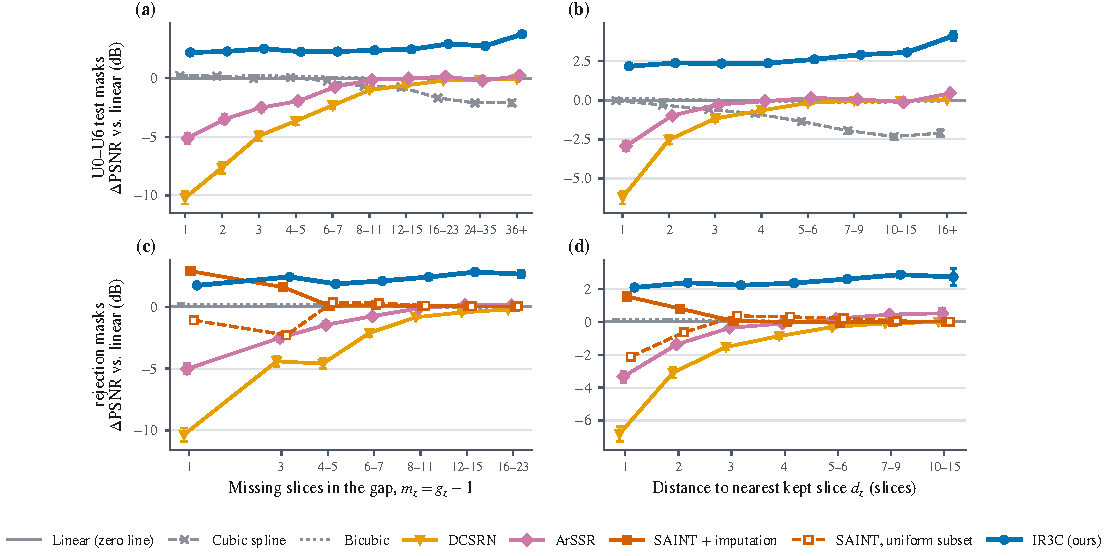
\includegraphics[width=\textwidth]{figs/fig8_gap.pdf}
\caption{Reconstruction error against local slice geometry on BraTS-GLI ($n=88$). Each
point is PSNR over the foreground of the missing slices in a bin, minus linear interpolation
on the same slices; squared error and voxel counts are pooled per subject and bin first, and
bars are 95\% confidence intervals across subjects. Rows: (a,b)~the 21 U0--U6 test masks at
$R\in\{2,4,8\}$; (c,d)~the 12 subject-specific rejection conditions. Columns: (a,c)~number of missing
slices in the gap, $m_z=g_z-1$; (b,d)~distance to the nearest kept slice $d_z$. Slices outside the outermost
kept slices and slices without foreground are excluded, and a bin is drawn only when at
least 20 subjects contribute. SAINT and I3Net run only on U0, so they are not drawn in (a,b);
on U0 alone SAINT is $+3.2$\,dB at $m_z=1$ (IR3C $+2.2$) and $+0.9$\,dB at $m_z=6$--7 (IR3C $+2.3$).}
\label{fig:gap}
\end{figure*}

\begin{pendingnote}{held-out geometry (Tables~\ref{tab:heldout} and \ref{tab:realisations})}
(i)~Train six IR3C models, each with one irregular family removed from the training
distribution, at the matched budget; evaluate each on its held-out family. The
``uniform-only'' column is the \texttt{C1\_uniform\_only} arm. (ii)~Generate five
subject-specific masks per family at $R=4$ (seed from the subject identifier and realisation
index) and re-score linear, bicubic, ArSSR, DCSRN and IR3C; inference only.
\end{pendingnote}

\begin{pendingnote}{additional baselines (shaded rows of Tables~\ref{tab:uniform} and \ref{tab:families})}
Add SA-INR \citep{wang2024sainr} under the matched protocol on all three datasets. It is the
closest published arbitrary-spacing method and appeared in this journal. The
``3D U-Net, direct output'' row is the \texttt{A3\_direct} arm, evaluated on all datasets.
\end{pendingnote}

\subsection{Computational cost}
\label{sec:res-cost}

IR3C reconstructs a BraTS-GLI volume in 0.26\,s, independently of $R$, because it processes
the whole volume in a single forward pass (Table~\ref{tab:cost}). DCSRN takes 1.2--2.6\,s.
ArSSR, \Ithree and SAINT take 2.9--14.3\,s, and their cost depends on the factor because they
run per slice or per query coordinate. IR3C is therefore 5--55 times faster than the learned
baselines. One IR3C model serves all factors and patterns, whereas DCSRN and \Ithree use a separate model for each factor.

\begin{table}[t]
\caption{Reconstruction time per BraTS-GLI volume ($240\times240\times153$), measured end to end on one NVIDIA GB10 GPU at fp32 with batch size 1. Times include patch extraction, sliding-window aggregation and output assembly, and are averaged over test volumes and three repetitions.}
\label{tab:cost}
\footnotesize\setlength{\tabcolsep}{3pt}
\begin{tabular*}{\columnwidth}{@{\extracolsep{\fill}}lcccc@{}}
\toprule
& & \multicolumn{3}{c}{Seconds per volume} \\
\cmidrule(lr){3-5}
Method & Params (M) & $R=2$ & $R=4$ & $R=8$ \\
\midrule
IR3C (ours) & 4.75 & 0.26 & 0.26 & 0.26 \\
DCSRN & 0.22 & 1.22 & 2.57 & 1.22 \\
ArSSR & 6.28 & 11.02 & 6.19 & 3.64 \\
I$^3$Net & 23.21 & 12.62 & 6.22 & 2.90 \\
SAINT & 3.16 & 14.26 & 8.60 & 6.01 \\
\bottomrule
\end{tabular*}
\end{table}


%% ================================================================= 6 DISCUSSION
\section{Discussion}
\label{sec:discussion}

\subsection{Principal finding}

The main result is a crossover between specialisation for a uniform grid and robustness to
the slice pattern. SAINT remains the better method at low sparsity on a uniform grid, and
clearly so on IXI-tiny. Once some acquired slices are rejected, however, the specialist
needs a workaround, and both workarounds give it an input that differs from what it was
trained on. IR3C applies the same inference procedure to whatever slices survive. Its
advantage appears at about 10\% rejection and grows with the rejected fraction. This is more
informative than marking an inapplicable method as ``not available'': both workarounds were
implemented and evaluated on identical missing slices.

\subsection{Why a simple formulation is sufficient}

IR3C does not owe its behaviour to a new architecture; its backbone is a standard 3D U-Net.
Two properties of the formulation explain what we observe. First, linear interpolation
already provides a good estimate in smooth regions and is exact at the kept slices, so the
network only needs to learn the departure from local linearity. The anchor ablation supports
this: the network absorbs most of a poor starting estimate, and the simplest anchor gives the
best final model. Second, the geometry profiles tell the network how far each missing slice
is from its neighbours and how long its gap is. The size of the correction a missing slice
needs depends on these quantities, and a network that sees them can adapt one set of weights
to any mask. DCSRN, which was trained on the same mixed masks without an anchor or explicit
geometry, gains little over linear interpolation. This suggests that mixed-mask training is
not sufficient on its own. A causal attribution to each component, however, requires the
formulation ablation in Table~\ref{tab:formulation}, which is pending.

The bound on the residual should be interpreted with care. It limits how far the output can
move from the anchor, but it does not guarantee a smaller error than linear interpolation. We
do not claim formal safety or non-degradation.

\subsection{Where IR3C should not be preferred}

On a uniform grid at low sparsity, a specialist such as SAINT is more accurate, by up to
3.7\,dB on IXI-tiny at $R=2$. If the slice pattern is guaranteed to be uniform and the
reduction factor is small, such a method is the better choice. IR3C should be preferred when
the slice pattern is irregular, when acquired slices may be rejected, when $R$ is large, or
when a reconstruction must be fast and feed a downstream analysis.

Brain-trained IR3C also does not transfer to knee MRI without fine-tuning; applied zero-shot,
it is worse than linear interpolation. The method is therefore flexible with respect to slice
geometry within a trained or adapted anatomy; it is not anatomy-invariant.

\subsection{Image metrics and downstream behaviour}
\label{sec:disc-metrics}

The segmentation experiment shows that PSNR should not be the only endpoint. SAINT and
\Ithree have reasonable PSNR but change the downstream segmentation substantially. The
classical interpolants trail by more than 2\,dB in PSNR yet remain close to IR3C on Dice,
because their errors are smooth. The loss-term ablation (Table~\ref{tab:loss}, pending)
tests the same point from the training side: if removing the background term leaves PSNR
almost unchanged but lowers Dice, PSNR is also an unreliable criterion for choosing the
training objective. The endpoint has a clear limitation: it measures
consistency with another model's prediction, not accuracy against expert labels.

LPIPS ranks the methods differently from every pixel metric (Table~\ref{tab:lpips}). On
OAIZIB, bicubic interpolation has about half the LPIPS of IR3C (0.184 versus 0.385) although it
is more than 2\,dB lower in PSNR. Learned reconstructions are smoother and closer to the
reference on average, whereas interpolation preserves high-frequency texture that a
natural-image feature space rewards even when that texture is misplaced
\citep{blau2018perception}. We therefore do not claim a perceptual advantage for IR3C.

\subsection{Limitations}
\label{sec:limitations}

This study has the following limitations. (i)~The degradation removes slices from a dense
reference and does not model slice profile, partial-volume averaging or slice gap; the
results concern slice imputation, not physical thick-slice super-resolution. (ii)~The
principal models use one training seed, so the paired confidence intervals describe
variation across subjects, not across training runs. (iii)~Checkpoint selection on
BraTS-GLI uses only six validation subjects. (iv)~The irregular test families are drawn from
the same generators as the training masks, and one mask per family is shared across subjects
(Section~\ref{sec:pending-heldout}). (v)~The downstream endpoint is consistency with a frozen
network rather than accuracy against expert labels. The labelled BraTS-GLI training release
was used in full to train the reconstruction models, so an accuracy evaluation would require
a new subject-level split and retraining every learned method. (vi)~In a voxel-based morphometry
analysis on IXI-tiny (not shown), IR3C reduced the area of significant grey-matter
differences compared with linear interpolation but introduced a one-signed underestimation
of total grey-matter volume, which validation-based calibration removed; IR3C should not be
used for volumetry without such calibration. (vii)~The rejection experiment covers the two
brain datasets; the knee arm is pending.

%% ================================================================= 7 CONCLUSION
\section{Conclusion}
\label{sec:conclusion}

Through-plane reconstruction methods should be evaluated on the slice patterns they will
receive, not only on uniform decimation. A specialist designed for a uniform grid can be the
most accurate method on that grid and still lose its advantage once a modest fraction of
acquired slices is rejected. IR3C combines a standard 3D U-Net with three simple ingredients:
an explicit description of the slice geometry, linear interpolation as an anchor, and exact
preservation of acquired slices. Across brain and knee MRI it is competitive on uniform
sampling, better than every applicable method on irregular sampling, more robust under slice
rejection, least disruptive to a downstream segmentation pipeline and 5--55 times faster than
the learned baselines. These results suggest that acquisition geometry deserves as much
attention as network architecture in missing-slice reconstruction.

%% ================================================================= DECLARATIONS
\section*{CRediT authorship contribution statement}
\authorfill{To be completed by the authors using the CRediT taxonomy.}

\section*{Declaration of competing interest}
The authors declare that they have no known competing financial interests or personal
relationships that could have appeared to influence the work reported in this paper.
\authorfill{Confirm.}

\section*{Data availability}
BraTS-GLI, IXI and Osteoarthritis Initiative data are available from their custodians under
their respective terms. Subject identifiers, split definitions, mask seeds and the
per-volume results used for every table and figure will be released with the code where
redistribution is permitted.

\section*{Code availability}
Training, inference, mask generation and evaluation code, with checkpoint provenance, will be
released upon publication. \authorfill{Repository URL or archive DOI.}

\section*{Declaration of generative AI use}
\authorfill{Elsevier requires this statement. During the preparation of this work the
authors used [tool names] in order to [purpose]. After using these tools, the authors reviewed
and edited the content as needed and take full responsibility for the content of the
published article.}

\section*{Acknowledgements}
The authors thank the organisers of BraTS, the IXI project and the Osteoarthritis Initiative,
and the developers of MONAI. \authorfill{Funding sources and grant numbers; computing support.}

\bibliographystyle{cas-model2-names}
\bibliography{references}

%% ================================================================= APPENDIX
\clearpage
\onecolumn
\appendix

\section{Detailed reconstruction results}
\label{app:detail}

Tables~\ref{tab:detail-brats}--\ref{tab:detailfam-ixi} give every distortion metric with
standard deviations for uniform sampling and PSNR with standard deviations for each family.
Means and standard deviations are computed across subjects after averaging within subject.
Table~\ref{tab:lpips} gives LPIPS.

\begin{table}[pos=!htbp]
\caption{BraTS-GLI, uniform sampling (U0), pooled over $R\in\{2,4,8\}$. Mean $\pm$ standard deviation across 88 test subjects, after averaging within subject. Bold marks the best method.}
\label{tab:detail-brats}
\small
\begin{tabular*}{\textwidth}{@{\extracolsep{\fill}}lcccc@{}}
\toprule
Method & PSNR (dB) $\uparrow$ & SSIM $\uparrow$ & NMSE $\downarrow$ & MAE $\downarrow$ \\
\midrule
Nearest & 22.80 $\pm$ 2.76 & 0.9463 $\pm$ 0.0215 & 0.0329 $\pm$ 0.0191 & 0.0463 $\pm$ 0.0187 \\
Linear & 26.20 $\pm$ 3.21 & 0.9545 $\pm$ 0.0202 & 0.0186 $\pm$ 0.0129 & 0.0320 $\pm$ 0.0171 \\
Cubic spline & 26.32 $\pm$ 3.31 & 0.9513 $\pm$ 0.0207 & 0.0191 $\pm$ 0.0140 & 0.0323 $\pm$ 0.0178 \\
Bicubic & 26.37 $\pm$ 3.28 & 0.9566 $\pm$ 0.0200 & 0.0186 $\pm$ 0.0134 & 0.0314 $\pm$ 0.0174 \\
DCSRN & 20.84 $\pm$ 1.79 & 0.8472 $\pm$ 0.0406 & 0.0467 $\pm$ 0.0297 & 0.0688 $\pm$ 0.0146 \\
ArSSR & 23.43 $\pm$ 2.40 & 0.9590 $\pm$ 0.0186 & 0.0253 $\pm$ 0.0115 & 0.0561 $\pm$ 0.0147 \\
I$^3$Net & 26.27 $\pm$ 3.01 & 0.9579 $\pm$ 0.0184 & 0.0179 $\pm$ 0.0116 & 0.0322 $\pm$ 0.0154 \\
SAINT & 28.39 $\pm$ 3.45 & 0.9670 $\pm$ 0.0167 & 0.0134 $\pm$ 0.0094 & 0.0259 $\pm$ 0.0141 \\
IR3C & \textbf{28.59 $\pm$ 3.59} & \textbf{0.9679 $\pm$ 0.0152} & \textbf{0.0118 $\pm$ 0.0089} & \textbf{0.0259 $\pm$ 0.0138} \\
\bottomrule
\end{tabular*}
\end{table}

\begin{table}[pos=!htbp]
\caption{BraTS-GLI, PSNR (dB) by sampling family, pooled over $R\in\{2,4,8\}$. Mean $\pm$ standard deviation across test subjects.}
\label{tab:detailfam-brats}
\footnotesize
\begin{tabular*}{\textwidth}{@{\extracolsep{\fill}}lccccccc@{}}
\toprule
Method & U0 & U1 & U2 & U3 & U4 & U5 & U6 \\
\midrule
Nearest & 22.80 $\pm$ 2.76 & 22.35 $\pm$ 2.75 & 21.85 $\pm$ 2.65 & 20.73 $\pm$ 2.54 & 16.68 $\pm$ 2.11 & 20.79 $\pm$ 2.49 & 19.60 $\pm$ 2.34 \\
Linear & 26.20 $\pm$ 3.21 & 25.03 $\pm$ 3.25 & 24.50 $\pm$ 3.10 & 23.12 $\pm$ 2.93 & 18.45 $\pm$ 2.36 & 23.37 $\pm$ 2.86 & 21.73 $\pm$ 2.66 \\
Cubic spline & 26.32 $\pm$ 3.31 & 24.96 $\pm$ 3.37 & 24.36 $\pm$ 3.26 & 22.53 $\pm$ 3.10 & 17.01 $\pm$ 2.55 & 22.96 $\pm$ 3.08 & 20.82 $\pm$ 2.94 \\
Bicubic & 26.37 $\pm$ 3.28 & 25.17 $\pm$ 3.33 & 24.61 $\pm$ 3.16 & 23.17 $\pm$ 2.99 & 18.46 $\pm$ 2.40 & 23.42 $\pm$ 2.90 & 21.78 $\pm$ 2.70 \\
DCSRN & 20.84 $\pm$ 1.79 & 20.64 $\pm$ 1.86 & 20.34 $\pm$ 1.85 & 19.78 $\pm$ 1.87 & 17.02 $\pm$ 1.82 & 19.77 $\pm$ 1.82 & 18.83 $\pm$ 1.75 \\
ArSSR & 23.43 $\pm$ 2.40 & 22.95 $\pm$ 2.51 & 22.65 $\pm$ 2.46 & 21.94 $\pm$ 2.46 & 18.14 $\pm$ 2.22 & 21.98 $\pm$ 2.39 & 20.51 $\pm$ 2.25 \\
IR3C & \textbf{28.59 $\pm$ 3.59} & \textbf{27.37 $\pm$ 3.62} & \textbf{26.84 $\pm$ 3.39} & \textbf{25.59 $\pm$ 3.17} & \textbf{21.42 $\pm$ 2.44} & \textbf{25.87 $\pm$ 3.11} & \textbf{24.27 $\pm$ 2.88} \\
\bottomrule
\end{tabular*}
\end{table}

\begin{table}[pos=!htbp]
\caption{OAIZIB, uniform sampling (U0), pooled over $R\in\{2,4,8\}$. Mean $\pm$ standard deviation across 103 test subjects, after averaging within subject. Bold marks the best method.}
\label{tab:detail-oaizib}
\small
\begin{tabular*}{\textwidth}{@{\extracolsep{\fill}}lcccc@{}}
\toprule
Method & PSNR (dB) $\uparrow$ & SSIM $\uparrow$ & NMSE $\downarrow$ & MAE $\downarrow$ \\
\midrule
Nearest & 17.57 $\pm$ 0.79 & 0.2676 $\pm$ 0.0228 & 0.1637 $\pm$ 0.0164 & 0.0915 $\pm$ 0.0099 \\
Linear & 19.19 $\pm$ 0.82 & 0.3103 $\pm$ 0.0256 & 0.1165 $\pm$ 0.0122 & 0.0789 $\pm$ 0.0085 \\
Cubic spline & 18.63 $\pm$ 0.84 & 0.2934 $\pm$ 0.0233 & 0.1322 $\pm$ 0.0140 & 0.0846 $\pm$ 0.0091 \\
Bicubic & 18.90 $\pm$ 0.83 & 0.3028 $\pm$ 0.0243 & 0.1248 $\pm$ 0.0132 & 0.0818 $\pm$ 0.0088 \\
DCSRN & 19.37 $\pm$ 0.72 & 0.2871 $\pm$ 0.0228 & 0.1089 $\pm$ 0.0117 & 0.0778 $\pm$ 0.0070 \\
ArSSR & 20.44 $\pm$ 0.84 & 0.3600 $\pm$ 0.0325 & 0.0853 $\pm$ 0.0093 & 0.0677 $\pm$ 0.0074 \\
I$^3$Net & 20.42 $\pm$ 0.84 & 0.3497 $\pm$ 0.0313 & 0.0867 $\pm$ 0.0097 & 0.0670 $\pm$ 0.0074 \\
SAINT & 21.35 $\pm$ 0.90 & 0.3979 $\pm$ 0.0317 & 0.0701 $\pm$ 0.0092 & 0.0609 $\pm$ 0.0071 \\
IR3C & \textbf{21.38 $\pm$ 0.90} & \textbf{0.4161 $\pm$ 0.0306} & \textbf{0.0684 $\pm$ 0.0091} & \textbf{0.0609 $\pm$ 0.0071} \\
\bottomrule
\end{tabular*}
\end{table}

\begin{table}[pos=!htbp]
\caption{OAIZIB, PSNR (dB) by sampling family, pooled over $R\in\{2,4,8\}$. Mean $\pm$ standard deviation across test subjects.}
\label{tab:detailfam-oaizib}
\footnotesize
\begin{tabular*}{\textwidth}{@{\extracolsep{\fill}}lccccccc@{}}
\toprule
Method & U0 & U1 & U2 & U3 & U4 & U5 & U6 \\
\midrule
Nearest & 17.57 $\pm$ 0.79 & 17.38 $\pm$ 0.78 & 17.27 $\pm$ 0.78 & 16.78 $\pm$ 0.75 & 14.84 $\pm$ 0.66 & 16.81 $\pm$ 0.79 & 16.23 $\pm$ 0.71 \\
Linear & 19.19 $\pm$ 0.82 & 18.68 $\pm$ 0.80 & 18.53 $\pm$ 0.80 & 18.03 $\pm$ 0.77 & 15.87 $\pm$ 0.68 & 18.07 $\pm$ 0.82 & 17.39 $\pm$ 0.72 \\
Cubic spline & 18.63 $\pm$ 0.84 & 17.71 $\pm$ 0.82 & 17.24 $\pm$ 0.82 & 15.45 $\pm$ 0.75 & 10.57 $\pm$ 0.58 & 14.67 $\pm$ 0.70 & 14.29 $\pm$ 0.74 \\
Bicubic & 18.90 $\pm$ 0.83 & 18.41 $\pm$ 0.81 & 18.27 $\pm$ 0.81 & 17.79 $\pm$ 0.78 & 15.71 $\pm$ 0.68 & 17.83 $\pm$ 0.82 & 17.18 $\pm$ 0.73 \\
DCSRN & 19.37 $\pm$ 0.72 & 18.98 $\pm$ 0.71 & 18.84 $\pm$ 0.70 & 18.35 $\pm$ 0.68 & 16.38 $\pm$ 0.63 & 18.40 $\pm$ 0.72 & 17.81 $\pm$ 0.65 \\
ArSSR & 20.44 $\pm$ 0.84 & 20.13 $\pm$ 0.83 & 19.99 $\pm$ 0.83 & 19.39 $\pm$ 0.80 & 16.90 $\pm$ 0.71 & 19.49 $\pm$ 0.86 & 18.78 $\pm$ 0.75 \\
IR3C & \textbf{21.38 $\pm$ 0.90} & \textbf{20.99 $\pm$ 0.87} & \textbf{20.88 $\pm$ 0.87} & \textbf{20.46 $\pm$ 0.85} & \textbf{18.59 $\pm$ 0.74} & \textbf{20.59 $\pm$ 0.89} & \textbf{19.94 $\pm$ 0.79} \\
\bottomrule
\end{tabular*}
\end{table}

\begin{table}[pos=!htbp]
\caption{IXI-tiny, uniform sampling (U0), pooled over $R\in\{2,4,8\}$. Mean $\pm$ standard deviation across 100 test subjects, after averaging within subject. Bold marks the best method.}
\label{tab:detail-ixi}
\small
\begin{tabular*}{\textwidth}{@{\extracolsep{\fill}}lcccc@{}}
\toprule
Method & PSNR (dB) $\uparrow$ & SSIM $\uparrow$ & NMSE $\downarrow$ & MAE $\downarrow$ \\
\midrule
Nearest & 19.85 $\pm$ 1.01 & 0.8097 $\pm$ 0.0119 & 0.0603 $\pm$ 0.0128 & 0.0621 $\pm$ 0.0111 \\
Linear & 23.07 $\pm$ 1.07 & 0.8464 $\pm$ 0.0101 & 0.0364 $\pm$ 0.0081 & 0.0460 $\pm$ 0.0083 \\
Cubic spline & 23.14 $\pm$ 1.15 & 0.8472 $\pm$ 0.0095 & 0.0394 $\pm$ 0.0081 & 0.0466 $\pm$ 0.0083 \\
Bicubic & 23.37 $\pm$ 1.12 & 0.8554 $\pm$ 0.0093 & 0.0365 $\pm$ 0.0080 & 0.0446 $\pm$ 0.0081 \\
DCSRN & 20.41 $\pm$ 0.93 & 0.7777 $\pm$ 0.0134 & 0.0579 $\pm$ 0.0152 & 0.0686 $\pm$ 0.0100 \\
ArSSR & 23.84 $\pm$ 1.52 & 0.9221 $\pm$ 0.0078 & 0.0232 $\pm$ 0.0025 & 0.0454 $\pm$ 0.0083 \\
I$^3$Net & 23.43 $\pm$ 1.09 & 0.8607 $\pm$ 0.0085 & 0.0335 $\pm$ 0.0070 & 0.0454 $\pm$ 0.0078 \\
SAINT & \textbf{27.81 $\pm$ 1.79} & \textbf{0.9405 $\pm$ 0.0058} & \textbf{0.0128 $\pm$ 0.0018} & \textbf{0.0271 $\pm$ 0.0055} \\
IR3C & 25.95 $\pm$ 1.41 & 0.9329 $\pm$ 0.0079 & 0.0154 $\pm$ 0.0023 & 0.0331 $\pm$ 0.0060 \\
\bottomrule
\end{tabular*}
\end{table}

\begin{table}[pos=!htbp]
\caption{IXI-tiny, PSNR (dB) by sampling family, pooled over $R\in\{2,4,8\}$. Mean $\pm$ standard deviation across test subjects.}
\label{tab:detailfam-ixi}
\footnotesize
\begin{tabular*}{\textwidth}{@{\extracolsep{\fill}}lccccccc@{}}
\toprule
Method & U0 & U1 & U2 & U3 & U4 & U5 & U6 \\
\midrule
Nearest & 19.85 $\pm$ 1.01 & 19.38 $\pm$ 1.00 & 19.41 $\pm$ 1.00 & 18.15 $\pm$ 1.02 & 13.35 $\pm$ 0.88 & 17.46 $\pm$ 1.02 & 17.10 $\pm$ 1.11 \\
Linear & 23.07 $\pm$ 1.07 & 21.45 $\pm$ 1.02 & 21.56 $\pm$ 1.03 & 19.93 $\pm$ 1.04 & 14.56 $\pm$ 0.85 & 19.25 $\pm$ 0.99 & 18.73 $\pm$ 1.23 \\
Cubic spline & 23.14 $\pm$ 1.15 & 21.36 $\pm$ 1.08 & 21.32 $\pm$ 1.06 & 18.66 $\pm$ 0.92 & 13.04 $\pm$ 0.87 & 15.06 $\pm$ 0.63 & 16.70 $\pm$ 1.13 \\
Bicubic & 23.37 $\pm$ 1.12 & 21.57 $\pm$ 1.03 & 21.69 $\pm$ 1.05 & 20.01 $\pm$ 1.04 & 14.56 $\pm$ 0.86 & 19.31 $\pm$ 1.00 & 18.72 $\pm$ 1.24 \\
DCSRN & 20.41 $\pm$ 0.93 & 19.71 $\pm$ 0.94 & 19.69 $\pm$ 0.97 & 18.70 $\pm$ 0.99 & 14.46 $\pm$ 0.82 & 18.27 $\pm$ 0.93 & 17.93 $\pm$ 1.17 \\
ArSSR & 23.84 $\pm$ 1.52 & 23.19 $\pm$ 1.54 & 23.12 $\pm$ 1.47 & 22.24 $\pm$ 1.44 & 17.36 $\pm$ 1.12 & 20.88 $\pm$ 1.46 & 21.86 $\pm$ 1.41 \\
IR3C & \textbf{25.95 $\pm$ 1.41} & \textbf{24.66 $\pm$ 1.35} & \textbf{24.69 $\pm$ 1.34} & \textbf{23.90 $\pm$ 1.28} & \textbf{20.26 $\pm$ 1.03} & \textbf{22.89 $\pm$ 1.23} & \textbf{23.25 $\pm$ 1.24} \\
\bottomrule
\end{tabular*}
\end{table}

\begin{table}[pos=!htbp]
\caption{LPIPS (AlexNet features, lower is better) on uniform sampling, pooled over $R\in\{2,4,8\}$, mean across test subjects. Learned methods are not better than classical interpolation on this metric (Section~\ref{sec:disc-metrics}). $^{\ddagger}$Full-budget IR3C; LPIPS was not computed for the matched-budget transfer models.}
\label{tab:lpips}
\footnotesize\setlength{\tabcolsep}{3pt}
\begin{tabular*}{\columnwidth}{@{\extracolsep{\fill}}lccc@{}}
\toprule
Method & BraTS-GLI & OAIZIB & IXI-tiny \\
\midrule
Linear & 0.0385 & 0.1916 & 0.0242 \\
Bicubic & \textbf{0.0347} & \textbf{0.1836} & 0.0196 \\
ArSSR & 0.0363 & 0.5491 & 0.0188 \\
I$^3$Net & --- & 0.4912 & 0.0273 \\
SAINT & 0.0388 & 0.4887 & \textbf{0.0176} \\
IR3C & 0.0376 & 0.3854$^{\ddagger}$ & 0.0190$^{\ddagger}$ \\
\bottomrule
\end{tabular*}
\end{table}


\FloatBarrier
\section{Slice rejection: absolute results}
\label{app:reject}

Tables~\ref{tab:reject-abs-brats} and \ref{tab:reject-abs-ixi} give the absolute PSNR of every
method in every rejection condition, including bicubic interpolation, DCSRN and both
workarounds for \Ithree and SAINT.

\begin{table}[pos=!htbp]
\caption{Slice rejection on BraTS-GLI: absolute PSNR (dB), mean across 88 test subjects. A: rejected slices imputed linearly, then the uniform-grid model is run at base $R$. B: the model is run at $2R$ on the uniform subset that lost fewer slices. Bold marks the best method per row.}
\label{tab:reject-abs-brats}
\footnotesize
\begin{tabular*}{\textwidth}{@{\extracolsep{\fill}}lllccccccccc@{}}
\toprule
Base & Pattern & Rejected & Linear & Bicubic & ArSSR & DCSRN & I$^3$Net-A & I$^3$Net-B & SAINT-A & SAINT-B & IR3C \\
\midrule
$R=2$ & --- & 0\% & 30.17 & 30.46 & 25.07 & 19.73 & 30.37 & 27.05 & \textbf{33.37} & 29.13 & 32.56 \\
$R=2$ & random & 10\% & 28.40 & 28.62 & 24.53 & 19.71 & 28.53 & 26.52 & 29.73 & 28.29 & \textbf{30.14} \\
$R=2$ & random & 20\% & 27.14 & 27.32 & 24.03 & 19.65 & 27.23 & 25.94 & 27.84 & 27.28 & \textbf{29.03} \\
$R=2$ & random & 30\% & 25.96 & 26.12 & 23.52 & 19.55 & 26.04 & 25.24 & 26.37 & 26.22 & \textbf{27.99} \\
$R=2$ & burst & 10\% & 27.12 & 27.30 & 24.03 & 19.56 & 27.22 & 25.66 & 28.13 & 26.81 & \textbf{28.74} \\
$R=2$ & burst & 20\% & 25.46 & 25.60 & 23.30 & 19.40 & 25.52 & 24.59 & 25.99 & 25.30 & \textbf{27.27} \\
$R=2$ & burst & 30\% & 24.09 & 24.19 & 22.55 & 19.19 & 24.14 & 23.61 & 24.37 & 24.03 & \textbf{26.09} \\
$R=4$ & --- & 0\% & 26.33 & 26.53 & 23.79 & 22.53 & 26.32 & 22.46 & 28.56 & 23.57 & \textbf{29.01} \\
$R=4$ & random & 10\% & 24.79 & 24.93 & 23.05 & 22.02 & 24.82 & 22.25 & 25.86 & 23.27 & \textbf{27.21} \\
$R=4$ & random & 20\% & 23.68 & 23.78 & 22.42 & 21.54 & 23.72 & 21.92 & 24.31 & 22.78 & \textbf{26.06} \\
$R=4$ & random & 30\% & 22.47 & 22.50 & 21.65 & 20.90 & 22.51 & 21.38 & 22.78 & 21.98 & \textbf{24.86} \\
$R=4$ & burst & 10\% & 24.08 & 24.17 & 22.58 & 21.66 & 24.11 & 21.81 & 25.05 & 22.60 & \textbf{26.60} \\
$R=4$ & burst & 20\% & 22.40 & 22.42 & 21.60 & 20.76 & 22.44 & 21.02 & 22.90 & 21.50 & \textbf{25.07} \\
$R=4$ & burst & 30\% & 21.10 & 21.09 & 20.70 & 19.96 & 21.14 & 20.30 & 21.38 & 20.53 & \textbf{23.69} \\
\bottomrule
\end{tabular*}
\end{table}

\begin{table}[pos=!htbp]
\caption{Slice rejection on IXI-tiny: absolute PSNR (dB), mean across 100 test subjects. A: rejected slices imputed linearly, then the uniform-grid model is run at base $R$. B: the model is run at $2R$ on the uniform subset that lost fewer slices. Bold marks the best method per row.}
\label{tab:reject-abs-ixi}
\footnotesize
\begin{tabular*}{\textwidth}{@{\extracolsep{\fill}}lllccccccccc@{}}
\toprule
Base & Pattern & Rejected & Linear & Bicubic & ArSSR & DCSRN & I$^3$Net-A & I$^3$Net-B & SAINT-A & SAINT-B & IR3C \\
\midrule
$R=2$ & --- & 0\% & 28.17 & 29.07 & 26.32 & 23.53 & 28.63 & 23.67 & \textbf{33.27} & 28.27 & 29.57 \\
$R=2$ & random & 10\% & 25.66 & 26.15 & 25.49 & 22.62 & 25.90 & 23.15 & \textbf{27.56} & 26.70 & 27.54 \\
$R=2$ & random & 20\% & 23.91 & 24.21 & 24.71 & 21.77 & 24.05 & 22.49 & 24.88 & 25.06 & \textbf{26.29} \\
$R=2$ & random & 30\% & 22.49 & 22.67 & 23.86 & 20.93 & 22.57 & 21.70 & 23.02 & 23.64 & \textbf{25.33} \\
$R=2$ & burst & 10\% & 24.73 & 25.09 & 24.95 & 22.12 & 24.90 & 22.52 & 26.15 & 25.26 & \textbf{26.93} \\
$R=2$ & burst & 20\% & 22.44 & 22.61 & 23.78 & 20.82 & 22.52 & 21.33 & 23.03 & 23.01 & \textbf{25.49} \\
$R=2$ & burst & 30\% & 20.98 & 21.07 & 22.81 & 19.86 & 21.02 & 20.38 & 21.31 & 21.50 & \textbf{24.51} \\
$R=4$ & --- & 0\% & 22.52 & 22.68 & 23.80 & 20.85 & 22.72 & 19.29 & \textbf{27.30} & 23.17 & 25.27 \\
$R=4$ & random & 10\% & 21.36 & 21.43 & 23.01 & 20.15 & 21.52 & 19.18 & 24.17 & 22.87 & \textbf{24.59} \\
$R=4$ & random & 20\% & 20.28 & 20.28 & 22.33 & 19.42 & 20.42 & 18.88 & 21.98 & 21.89 & \textbf{23.97} \\
$R=4$ & random & 30\% & 19.21 & 19.14 & 21.48 & 18.63 & 19.32 & 18.40 & 20.16 & 20.57 & \textbf{23.32} \\
$R=4$ & burst & 10\% & 20.73 & 20.75 & 22.64 & 19.69 & 20.87 & 18.73 & 22.85 & 21.43 & \textbf{24.30} \\
$R=4$ & burst & 20\% & 19.61 & 19.57 & 21.62 & 18.91 & 19.73 & 18.33 & 20.86 & 20.53 & \textbf{23.53} \\
$R=4$ & burst & 30\% & 18.36 & 18.26 & 20.65 & 17.92 & 18.45 & 17.62 & 19.04 & 19.05 & \textbf{22.80} \\
\bottomrule
\end{tabular*}
\end{table}


\FloatBarrier
\section{Training budget}
\label{app:budget}

Table~\ref{tab:budget} compares the matched-budget IR3C used throughout with the full-budget
model. The matched model is 0.45\,dB lower on BraTS-GLI, so the matched comparison does not
favour IR3C. On the transfer datasets, the source checkpoint used to initialise fine-tuning
has almost no effect.

\begin{table}[pos=!htbp]
\caption{Effect of the source training budget on IR3C (PSNR in dB, all families, $R\in\{2,4,8\}$). ``Matched'' stops source training at 12,510 steps, the largest budget given to any baseline, and is the model used in every comparison. ``Full'' uses the complete 25-epoch schedule (selected at step 28,773). For OAIZIB and IXI-tiny, the two rows differ only in the source checkpoint used to initialise fine-tuning.}
\label{tab:budget}
\footnotesize\setlength{\tabcolsep}{3pt}
\begin{tabular*}{\columnwidth}{@{\extracolsep{\fill}}lccc@{}}
\toprule
Dataset & Matched & Full & Full $-$ matched \\
\midrule
BraTS-GLI & 25.71 & 26.16 & $+$0.45 [0.42, 0.48] \\
OAIZIB & 20.40 & 20.40 & 0.00 [$-$0.01, 0.00] \\
IXI-tiny & 23.66 & 23.75 & $+$0.10 [0.09, 0.10] \\
\bottomrule
\end{tabular*}
\end{table}


\FloatBarrier
\clearpage
\end{document}
